% !Mode:: "Tex:UTF-8"
\chapter{面向流控机制的对偶综合}
\label{chap:6}

%在假设一个编码器的输入总能够被其输出完全唯一决定的前提下,
%传统对偶综合算法能够自动化的生成一个编码器的解码器。
%然而,为了防止快速的编码器发送过多数据以至于解码器无法处理,
%许多通讯协议的编码器采用了流控机制\upcite{flowcontrol}。
%当编码器发送的数据流过快以至于无法被解码器处理时,
%这些编码器将停止发送数据,
%而改为发送空闲字符,
%而这些空闲字符无法用于唯一决定编码器的输入信号。
%在这种情况下,
%解码器应当识别并淘汰这些空闲信号。
%虽然流控机制能够避免丢失数据,
%但是他却直接违反了目前所有对偶综合算法的前提假设,
%即一个编码器的输入应当能够被其输出唯一决定。
%
%本文提出了首个能够处理流控机制的对偶综合算法。
%该算法首先识别所有能够被唯一决定的输入变量,
%并将他们视为流控变量。
%其次,该算法在这些流控变量上推导一个能够使得其他变量被唯一决定的谓词。
%最后,使用Craig插值算法产生所有流控变量的解码函数。
%而对于非流控变量,
%在使用Craig插值算法之前,在第二步中被推导出来的谓词应该首先被应用。
%
%本章从理论和实验两方面证明了该算法的正确性和有效性。

\section{ 引言}

在通讯和多媒体芯片设计中,
一个最为困难且容易出错的工作就是设计该协议的的编码器和解码器。
其中编码器将输入变量$\vec{i}$映射到输出变量$\vec{o}$.
而解码器则从$\vec{o}$中恢复$\vec{i}$。
对偶综合算法
\upcite{ShenICCAD09,ShenTCAD10,ShenTCAD11,ShenICCAD11,ShenTCAD12,LiuICCAD11,LiuTCAD12,TuDAC13}
通过自动生成特定编码器的解码器以降低该工作的复杂度并提高结果的可靠性。
该算法的一个前提假设是,
编码器的输入变量$\vec{i}$总能够被输出变量$\vec{o}$的一个有限长度序列唯一决定。

然而,
许多高速通讯系统的编码器带有流控功能\upcite{flowcontrol},
而该功能直接违反了上述假设。
图\ref{fig:nonuniq}a)展示了一个带有流控机制的通讯系统的结构。
其中一个传输器(transmitter)和一个接收器(receiver)通过一个编码器(encoder)和一个解码器(decoder)连接在一起。
从传输器到编码器有两个输入变量:
有待编码的数据位$d$,
和代表$d$的有效性的有效位$f$。
图\ref{fig:nonuniq}b)给出了编码器如何将
$f$和$d$映射到输出变量$\vec{o}$的编码表。

流控机制的工作原理为:
\begin{enumerate}
\item
当接收器能够跟上发送器的速度时,
发送器将$f$设为1,
这使得编码器按照$d$的值发送$D_d$。
从图\ref{fig:nonuniq}b)的编码表可知,
解码器总能够根据$D_d$恢复$f$和$d$。
\item
而当接收器无法跟上发送器的速度时,
发送器将$f$设为0以阻止编码器继续发送$D_d$,
转而在不考虑$d$的情况下发送空闲符号$I$。
而解码器应当识别并淘汰$I$,
并将$f\equiv 0$发送给接收器。
此时$d$的具体值并不重要。
\end{enumerate}

上述流控机制能够防止快速发送器发送过多数据以至于接收器无法处理。
然而该机制违反了迄今为止所有对偶综合算法
\upcite{ShenICCAD09,ShenTCAD10,ShenTCAD11,ShenTCAD12,LiuICCAD11,LiuTCAD12,TuDAC13}
的基本假设,
因为$d$无法被$I$唯一决定。
很明显,
为了解决该问题,
我们只需考虑$f\equiv 1$的情形,
因为在此情况下$d$是能够被唯一决定的。
而对于$f\equiv 0$的情况,
$d$是无意义的,可以无需考虑。

\begin{figure}
\centerline{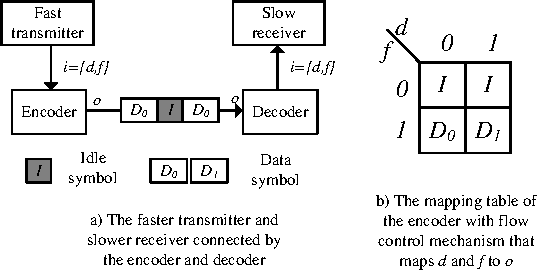
\includegraphics[width=\textwidth]{nonuniq}}
\caption{带有流控机制的通讯系统及其编码器}
\label{fig:nonuniq}
\end{figure}


基于上述讨论,
本文提出了首个能够处理流控机制的对偶综合算法。
该算法分为三步:
首先,
该算法使用算法\ref{alg_pcln_chap1}发掘所有能够被唯一决定的输入变量,
并将它们作为流控向量$\vec{f}$。
其次,
该算法在$\vec{f}$上特征化一个流控谓词$valid(\vec{f})$,
使得剩余的所有输入变量均能被输出唯一决定。
最后,
该算法产生解码器的布尔函数。

该算法的第二步类似于\upcite{ShenTCAD12},
因为他们都试图得到使得$\vec{d}$或者$\vec{i}$被唯一决定的谓词。
然而他们的根本区别在于
\upcite{ShenTCAD12}的算法推导的是一个全局谓词,
必须在整个展开的迁移关系上都成立。
% so that the encoder eventually reaches and never leaves the unique state set,
而本文算法得到的是仅应用于当前步的谓词,以恢复$\vec{d}$。
因此本文算法可以视为\upcite{ShenTCAD12}的一般化。

实验结果表明,
对于多个来自于工业界的复杂编码器(如以太网 \upcite{IEEE8023_S4}和PCI Express \upcite{pcie21}),
本文算法总能够正确的识别流控变量$\vec{f}$,
推导谓词$valid(\vec{f})$,
并产生解码器。
同时,
我们也和现有算法进行了运行时间,电路面积和时序方面的比较。



\emph{本章剩余部分按照以下方式组织}。
%Section \ref{sec_casestudy} explains our ideas with a simple example。
%第\ref{sec_prem}节介绍了背景知识;
第\ref{sec_findfc}节给出了识别流控变量的算法,
而第\ref{sec_infer}节推导使得$\vec{d}$能够被$\vec{o}$唯一决定的谓词;
第\ref{sec_min}节压缩迁移关系展开的长度以降低运行时间并减小电路面积和延时,
而第\ref{sec_char_chap3}节给出了特征化解码器电路的算法;
第\ref{sec_exp_chap3}和\ref{sec_conclude_chap3}节分别给出了实验结果和结论。



%
%\section{背景知识}\label{sec_prem}
%本节介绍相关的背景知识。
%\subsection{命题逻辑可满足问题}\label{subsec_SAT}
%布尔集合记为$B=\{0,1\}$。
%多个变量组成的向量记为$\vec{v}=(v,\dots)$。
%$\vec{v}$中的变量个数记为$|\vec{v}|$。
%如果$v$是$\vec{v}$的成员,
%则记为$v\in\vec{v}$;
%否则$v\notin\vec{v}$。
%对于变量$v$和向量$\vec{v}$,
%如果$v\notin\vec{v}$,
%则同时包含$v$和所有$\vec{v}$的成员的新向量记为$v\cup\vec{v}$。
%如果$v\in \vec{v}$,
%则包含所有$\vec{v}$的成员而不包含$v$的新向量记为$\vec{v}-v$。
%对于两个向量$\vec{a}$和$\vec{b}$,
%包含$\vec{a}$和$\vec{b}$的所有成员的新向量记为$\vec{a}\cup\vec{b}$。
%向量$\vec{v}$的赋值集合记为$[\![\vec{v}]\!]$。
%例如:
%$[\![(v_1,v_2)]\!]=\{(0,0),(0,1),(1,0),(1,1)\}$。
%
%在变量集合$V$上的布尔逻辑公式$F$是通过以下连接符连接$V$上的变量得到的:
%包括$\neg$, $\wedge$, $\vee$和$\Rightarrow$,
%他们分别代表着求反,与,或和蕴含操作。
%
%对在变量集合$V$上的布尔逻辑公式$F$,
%命题逻辑可满足问题(缩写为SAT)
%意味着寻找$V$的赋值函数$A:V\to B$,
%使得$F$ 可以取值为$1$。
%如果存在这样的赋值函数$A$,
%则$F$ 是可满足的;
%否则,
%是不可满足的。
%
%一个寻找上述赋值函数$A$的计算机程序称为SAT 求解器,
%常见的SAT求解器包括Zchaff\upcite{CHAFF},
%Grasp\upcite{grasp},
%Berkmin\upcite{BERKMIN},
%和MiniSat\upcite{EXTSAT}。
%
%
%通常,
%SAT 求解器要求有待求解的公式使用合取范式(CNF)表示,
%其中一个公式是一个短句集合的合取,
%一个短句是一个文字集合的析取,
%一个文字是一个变量或者其反。
%一个使用CNF 格式表示的公式通常也称为SAT 实例。
%
%
%从文献\upcite{EFFSATUSMCCO}可知,
%对于函数$f(v_1\dots v\dots v_n)$,
%针对变量$v$的正cofactor和负cofactor分别是$f_{v\equiv 1}=f(v_1\dots 1\dots v_n)$和$f_{v\equiv 0}=f(v_1\dots 0\dots v_n)$。
%而Cofactoring则代表着将1或者0赋予$v$以得到$f_{v\equiv 1}$ 和$f_{v\equiv 0}$。
%
%给定两个布尔逻辑公式$\phi_A$ 和$\phi_B$,
%若$\phi_A\wedge \phi_B$ 不可满足,
%则存在仅使用了$\phi_A$ 和$\phi_B$共同变量的公式$\phi_I$ ,
% 使得$\phi_A\Rightarrow \phi_I$且
%$\phi_I\wedge \phi_B$不可满足。
%$\phi_I$ 被称为$\phi_A$针对$\phi_B$的Craig插值\upcite{Craig}。
%$\phi_I$可以使用McMillan算法\upcite{interp_McMillan}得到。
%Craig插值通常被用于产生$\phi_A$的上估计。
%
%
%\subsection{MiniSat 求解器的递增求解机制}\label{subsec_incsat}
%
%本文中,
%我们使用MiniSat 求解器\upcite{EXTSAT} 求解所有CNF公式。
%和其他基于冲突学习机制\upcite{CONFLICTLEARN}的SAT求解器类似,
%MiniSat 从在搜索中遇到的冲突中产生学习短句,
%并记录他们以避免类似的冲突再次出现。
%该机制能够极大的提升SAT求解器的性能。
%
%在许多应用中,
%经常存在一系列紧密关联的CNF公式。
%如果在一个CNF公式求解过程中得到的学习短句能够被其他CNF公式共享,
%则所有CNF公式的求解速度都能够得到极大的提升。
%
%MiniSat 提供了一个增量求解机制以共享这些学习短句。
%该机制包括两个接口函数:
%\begin{enumerate}
%\item
%$addClause(F)$ 用于将一个CNF公式$F$ 添加到MiniSat的短句数据库,
%以用于下一轮求解。
%\item
%$solve(A)$ 接收一个文字集合$A$作为假设,
%并求解CNF 公式$F\wedge \bigwedge_{a\in A} a$。
%其中$F$是在$addClause$中被加入短句数据库的CNF公式。
%\end{enumerate}
%
%
%\subsection{有限状态机}
%
%本文中编码器使用有限状态机$M=(\vec{s},\vec{i},\vec{o},T)$作为模型。
%一个状态机包括状态变量向量$\vec{s}$,
%输入变量向量$\vec{i}$,
%输出变量向量$\vec{o}$,
%和迁移函数$T: [\![\vec{s}]\!]\times [\![\vec{i}]\!]\to [\![\vec{s}]\!]\times [\![\vec{o}]\!]$。
%其中$T$用于从当前状态变量向量$\vec{s}$和输入变量向量$\vec{i}$计算出下一状态变量向量$\vec{s}$和输出变量向量$\vec{o}$。
%
%有限状态机$M$的行为可以通过将迁移函数展开多步得到。
%在第n步上,
%状态变量$s\in\vec{s}$,输入变量$i\in\vec{i}$ 和输出变量$o\in\vec{o}$
%分别表示为$s_n$,$i_n$ 和 $o_n$。
%进一步的,
%在第n步的状态变量向量,输入变量向量和输出变量向量分别记为$\vec{s}_n$,$\vec{i}_n$ 和 $\vec{o}_n$。
%一条路径是一个状态序列$<\vec{s}_n,\dots,\vec{s}_m>$ 使得$\exists \vec{i}_j\vec{o}_j (\vec{s}_{j+1},\vec{o}_j)\equiv T(\vec{s}_j,\vec{i}_j)$ 对所有$n\le j< m$均满足。
%一个环是一条路径$<\vec{s}_n,\dots,\vec{s}_m>$使得$\vec{s}_n\equiv \vec{s}_m$。
%
%\subsection{确认一个输入变量是否能够被输出变量的有限长序列唯一决定的停机算法}\label{subsec_chkextdec}
%
%目前所有的对偶综合算法
%\upcite{ShenICCAD09,ShenTCAD10,ShenTCAD11,ShenTCAD12,LiuICCAD11,LiuTCAD12,TuDAC13}
%均假设$\vec{i}$能够被输出变量的有限长序列唯一决定,
%因此他们均将$\vec{i}$ 视为一个整体,
%而不单独考虑每个$i\in\vec{i}$。
%然而在本文中,
%我们需要检查每一个单独的$i\in\vec{i}$ 。
%因此本文的表达方式有可能和现有算法
%\upcite{ShenICCAD09,ShenTCAD10,ShenTCAD11,ShenTCAD12,LiuICCAD11,LiuTCAD12,TuDAC13}
%存在细微差别。
%
%我们在文献\upcite{ShenTCAD11}中提出了第一个完成此任务的停机算法。
%其基本思想是将迁移函数展开至递增的长度序列。
%而对于每一个展开长度,
%使用两个近似估计算法以获得当前的答案。
%第一个估计算法是第\ref{subsub_sound}节中描述的下估计算法。
%而第二个估计算法是第\ref{subsub_complete}节中描述的上估计算法。
%因此,
%当第一个算法给出的答案是"是"的时候,则最终答案也是"是",
%当第二个算法给出的答案是"否"的时候,则最终答案也是"否"。
%我们将在第\ref{subsub_algo} 节中证明这两个算法随着展开长度的增长必将收敛并停机,
%并给出确定的答案。
%
%\subsubsection{下估计算法}\label{subsub_sound}
%
%如图\ref{fig_pc}所示,
%在展开的迁移函数序列上,
%如果存在三个参数$p$, $l$ 和$r$,
%使得对于输出序列$<\vec{o}_p,\dots,\vec{o}_{p+l+r}>$的任意取值,
%$i_{p+l}$不能同时取值为0和1,
%则输入变量$i\in\vec{i}$可以被唯一决定。
%这等价于等式(\ref{uniqt1})中的公式$F_{PC}(p,l,r)$的不可满足。
%
%\begin{equation}\label{uniqt1}
%% \begin{split}
%F_{PC}(p,l,r):=
%\left\{
%\begin{array}{cc}
%&\bigwedge_{m=0}^{p+l+r}
%\{
%(\vec{s}_{m+1},\vec{o}_m)\equiv T(\vec{s}_m,\vec{i}_m)
%\}
%\\
%\wedge&\bigwedge_{m=0}^{p+l+r}
%\{
%(\vec{s'}_{m+1},\vec{o'}_m)\equiv T(\vec{s'}_m,\vec{i'}_m)
%\}
%\\
%\wedge&\bigwedge_{m=p}^{p+l+r}\vec{o}_m\equiv \vec{o'}_m \\
%\wedge& i_{p+l}\equiv 1 \wedge  i'_{p+l}\equiv 0 \\
%\wedge&\bigwedge_{m=0}^{p+l+r}assertion(\vec{i}_m) \\
%\wedge&\bigwedge_{m=0}^{p+l+r}assertion(\vec{i'}_m)
%\end{array}
%\right\}
%% \end{split}
%\end{equation}
%
%\begin{figure}[b]
%\begin{center}
%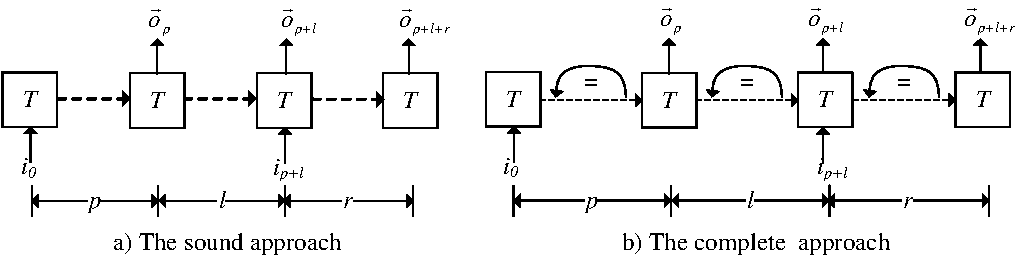
\includegraphics[width=\textwidth]{pc}
%\end{center}
%\caption{用于检查$i_{p+l}$ 是否能够被唯一决定的下估计算法}
%  \label{fig_pc}
%\end{figure}
%
%
%这里,
%$p$是前置迁移函数序列的长度,
%$l$ 和$r$则是两个用于唯一决定$i_{p+l}$的输出序列
%$<\vec{o}_{p+1},\dots,\vec{o}_{p+l}>$ 和$<\vec{o}_{p+l+1},\dots,\vec{o}_{p+l+r}>$
%的长度。
%等式(\ref{uniqt1}) 的行1对应于图\ref{fig_pc}左边的路径,
%而行2对应于图\ref{fig_pc}右边的路径。
%他们的长度是相同的。
%行3强制这两条路径的输出是相同的。
%而行4要求他们的输入$i_{p+l}$ 是不同的。
%行5和6则是用户给出的断言,
%用于约束合法的输入模式。
%$F_{PC}$ 中的PC是"parameterized complementary"的缩写,
%意味着$F_{PC}(p,l,r)$ 被用于检查在三个参数 $p$,$l$ 和 $r$的情况下,
%$i_{p+l}$能否被唯一决定。
%
%
%从图\ref{fig_pc}可知,
%等式(\ref{uniqt1}) 的前三行代表了两个具有相同输出的迁移函数展开序列。
%因此他们总是可满足的。
%而最后两行是对合法输入模式的约束。
%我们将在算法开始前检查他们的可满足性。
%所以$F_{PC}(p,l,r)$ 的不可满足意味着$i_{p+l}\equiv i'_{p+l}$,
%即输入被唯一决定。
%
%从图\ref{fig_pc}可知,
%如果$F_{PC}(p,l,r)$ 不可满足
%则$F_{PC}(p',l',r')$ 对于更大的$p'\ge p$, $l'\ge l$ 和$r'\ge r$也不可满足。
%从等式(\ref{uniqt1})中可知,
%$F_{PC}(p',l',r')$ 的短句集合是$F_{PC}(p,l,r)$的超集。
%这也指向了同一个结论。
%
%这意味着,
%$F_{PC}(p,l,r)$的不可满足性的限界证明可以被扩展到
%任意$p$, $l$ 和$r$上,
%从而成为非限界的证明。
%
%\begin{proposition}\label{prop_pc1}
%如果$F_{PC}(p,l,r)$ 不可满足
%则对于任意更大的$p$, $l$ 和$r$,
%$i_{p+l}$ 能够被$<\vec{o}_{p},\dots,\vec{o}_{p+l+r}>$ 唯一决定。
%\end{proposition}
%
%等式(\ref{uniqt1}) 不包含初始状态,
%相反使用一个长度为$p$步的前置状态序列$<\vec{s_0},\dots,\vec{s_{p-1}}>$
%以将约束$assertion(\vec{i})$传播到状态序列$<\vec{s_p},\dots,\vec{s_{p+l+r}}>$。
%从而将在$assertion(\vec{i})$ 约束下不可达的状态集合剔除。
%相比考虑初始状态的传统方法,这带来了两个主要的好处:
%首先,
%通过不计算可达状态,
%本文算法可以得到极大的简化和加速。
%而相比之下,目前唯一能够计算可达状态的对偶综合算法\upcite{TuDAC13}
%则无法处理最为复杂的XFI编码器。
%而我们的算法\upcite{ShenTCAD11}则始终可以处理。
%第二,
%通过忽略初始状态,本文算法可以提升产生出来的解码器的可靠性。
%因为这可以使得解码器的状态和输出仅仅依赖于有限的输入历史。
%因此任何被传输中的错误破坏的$\vec{o}$ 只能对解码器产生有限步数的影响。
%
%当然忽略初始状态有一个缺点在于,
%他使得判断条件比必须的情况稍微强一些。
%也就是说,
%他要求$\vec{i}$ 必须在一个更大的集合$R^p$上被唯一决定。
%其中$R^p$代表了由任意状态在$p$步之内能够到达的状态集合。
%而必要条件是从初始条件出发在任意步数内可以到达的可达状态集合$R$。
%因此在某些情况下,
%我们的算法有可能无法处理正确设计的编码器。
%不过从目前使用的所有编码器,即使是那些来自于真实工业应用的编码器,
%这种极端情况也没有出现过。
%
%
%\subsubsection{上估计算法}\label{subsub_complete}.
%
%在上一小节,
%我讨论了当$F_{PC}(p,l,r)$ 不可满足时,
%$i_{p+l}$能够针对任意$p$, $l$ 和$r$被唯一决定。
%另一方面,
%如果$F_{PC}(p,l,r)$ 是可满足的,
%则$i_{p+l}$ 不能在特定的$p$, $l$ 和$r$情况下被$<\vec{o}_{p},\dots,\vec{o}_{p+l+r}>$ 唯一决定。
%此时存在两种可能性:
%\begin{enumerate}
% \item
%在更大的$p$, $l$ 和$r$情况下$i_{p+l}$能够被$<\vec{o}_{p},\dots,\vec{o}_{p+l+r}>$ 唯一决定。
% \item
%对任意$p$, $l$ 和$r$,$i_{p+l}$ 都不能够被$<\vec{o}_{p},\dots,\vec{o}_{p+l+r}>$ 唯一决定。
%\end{enumerate}
%
%如果是第一种情况,
%则通过迭代的增长$p$, $l$ 和$r$,
%$F_{PC}(p,l,r)$ 总能够变成不可满足。
%然而对于第二种情况,
%迭代的递增$p$, $l$ 和$r$将导致不停机。
%
%\begin{figure}[b]
%\begin{center}
%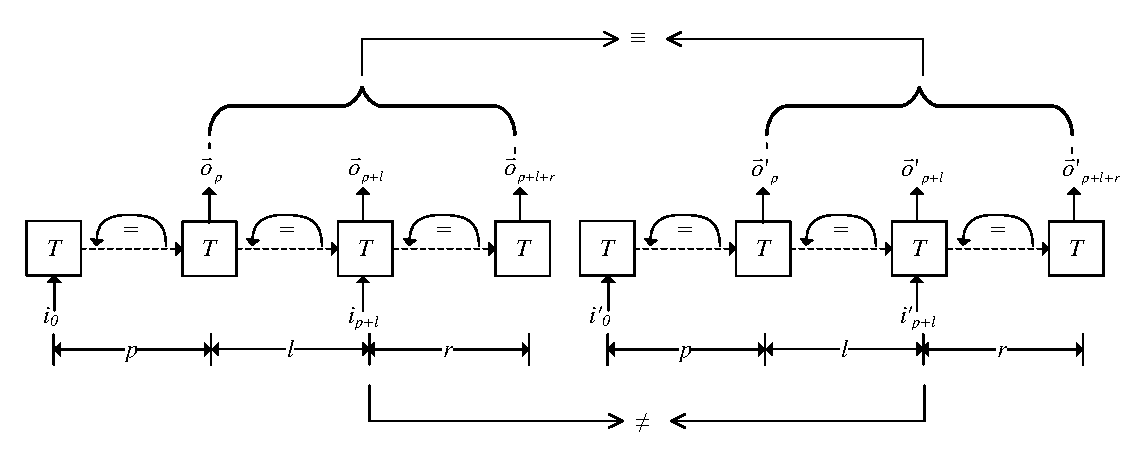
\includegraphics[width=\textwidth]{ln}
%\end{center}
%\caption{用于检查$i_{p+l}$ 是否不能被唯一决定的上估计算法}
%  \label{fig_ln}
%\end{figure}
%
%因此,
%为了得到一个停机算法,
%我们需要区分上述两种情形的手段。
%该手段如图\ref{fig_ln}所示,
%该图类似于图\ref{fig_pc},
%但是增加了三个约束用于检测三个路径$<\vec{s}_{0},\dots,\vec{s}_{p}>$,$<\vec{s}_{p+1},\dots,\vec{s}_{p+l}>$ 和
%$<\vec{s}_{p+l+1},\dots,\vec{s}_{p+l+r}>$上的环。
%该方法被形式化的定义于等式(\ref{uniqln}) 中。
%
%\begin{equation}\label{uniqln}
%% \begin{split}
%F_{LN}(p,l,r):=\\
%\left\{
%\begin{array}{cc}
%&F_{PC}(p,l,r)\\
%\wedge&\bigvee_{x=0}^{p-1}\bigvee_{y=x+1}^{p} \{\vec{s}_x\equiv \vec{s}_y\wedge \vec{s'}_x\equiv \vec{s'}_y\} \\
%\wedge&\bigvee_{x=p+1}^{p+l-1}\bigvee_{y=x+1}^{p+l} \{\vec{s}_x\equiv \vec{s}_y\wedge \vec{s'}_x\equiv \vec{s'}_y\} \\
%\wedge&\bigvee_{x=p+l+1}^{p+l+r-1}\bigvee_{y=x+1}^{p+l+r} \{\vec{s}_x\equiv \vec{s}_y\wedge \vec{s'}_x\equiv \vec{s'}_y\}
%\end{array}
%\right\}
%% \end{split}
%\end{equation}
%
%$F_{LN}$ 中的LN意味着环形非对偶。
%这表明$F_{LN}(p,l,r)$ 将使用这三个环检测约束来检测$i_{p+l}$是否不能够被唯一决定。
%
%当$F_{LN}(p,l,r)$ 可满足,
%则$i_{p+l}$ 不能被$<\vec{o}_{p},\dots,\vec{o}_{p+l+r}>$唯一决定。
%更重要的,
%通过展开这三个环,
%我们能将这个结论扩展到任意更大的$p$, $l$ 和$r$上。
%这意味着:
%
%\begin{proposition}\label{prop_ln1}
%当$F_{LN}(p,l,r)$ 可满足时,
%$i_{p+l}$ 针对任意$p$, $l$ 和$r$都不能被$<\vec{o}_{p},\dots,\vec{o}_{p+l+r}>$ 唯一决定。
%\end{proposition}
%
%\subsubsection{完整算法}\label{subsub_algo}.
%
%
%\begin{algorithm}[t]
%\caption{$CheckUniqueness(i)$:用于检测$i\in\vec{i}$是否能够被$\vec{o}$的有限长度序列唯一决定的停机算法}
%\label{alg_pcln}
%\begin{algorithmic}[1]
%\STATE $p$:= 0; ~$l$:= 0;~$r$:= 0
%\WHILE {$1$}
%\STATE $p$++;~$l$++;~$r$++ ;
%\IF{$F_{PC}(p,l,r)$ 不可满足}\label{linepc1}
%\RETURN ($1$,$p$,$l$,$r$)\label{lineln1};
%\ELSIF{$F_{LN}(p,l,r)$ 可满足}\label{lnsat}
%\RETURN ($0$,$p$,$l$,$r$);
%\ENDIF
%\ENDWHILE
%\end{algorithmic}
%\end{algorithm}
%
%%
%%\KwIn{The input variable $i\in\vec{i}$.}
%%\KwOut{whether $i\in\vec{i}$ can be uniquely determined by $\vec{o}$, and the value of $p$, $l$ and $r$.}
%
%
%
%
%根据命题\ref{prop_pc1} 和\ref{prop_ln1},
%我们能将针对特定$p$, $l$ 和$r$的限界证明扩展到针对任意$p$, $l$ 和$r$的非限界情形。
%这使得我们得到停机算法\ref{alg_pcln},
%用于检测$i\in\vec{i}$是否能被$\vec{o}$的有限长度序列唯一决定。
%\begin{enumerate}
% \item
%一方面,
%如果确实存在$p$, $l$ 和$r$,使得输入能被输出唯一决定,
%令$p':=max(p,l,r)$,$l':=max(p,l,r)$ 和$r':=max(p,l,r)$。
%从命题\ref{prop_pc1},
%可知$F_{PC}(p',l',r')$ 是不可满足的。
%因此$F_{PC}(p,l,r)$ 总能够在算法\ref{alg_pcln}行\ref{linepc1}成为不可满足的并退出循环;
% \item
%另一方面,
%如果不存在这样的$p$, $l$ 和$r$,
%则$p$, $l$ 和$r$ 在不断的递增之后最终总能够大于有限状态机的最大无环路径长度。
%这意味着在$<\vec{s}_{0},\dots,\vec{s}_{p}>$,$<\vec{s}_{p+1},\dots,\vec{s}_{p+l}>$ 和
%$<\vec{s}_{p+l+1},\dots,\vec{s}_{p+l+r}>$上都存在环。
%这将使得$F_{LN}(p,l,r)$ 在行\ref{lnsat}被满足。这样将导致退出循环。
%\end{enumerate}
%
%
%因此该算法是停机的。



\section{识别流控变量}\label{sec_findfc}
本节将介绍如何识别流控变量$\vec{f}$。
这将首先在小节\ref{basic}中介绍。
然后小节\ref{incSAT}将介绍如何使用增量求解算法加速该算法。

\subsection{识别流控变量$\vec{f}$}\label{basic}

为了便于描述,
我们假设$\vec{i}$ 可以被划分为两个向量:
流控向量$\vec{f}$ 和数据向量$\vec{d}$。

流控向量$\vec{f}$ 用于表达$\vec{d}$的有效性。
所以对于一个正确设计的编码器,
$\vec{f}$ 总能够被输出变量向量$\vec{o}$的一个有限长度序列唯一决定。
否则解码器无法识别$\vec{d}$的有效性。


\begin{algorithm}[b]
\caption{$FindFlow(\vec{i})$:识别$\vec{f}$}
\label{alg_fofc}
%\SetAlgoVlined
%\KwIn{The input variable vector $\vec{i}$.}
%\KwOut{$\vec{f}\subset \vec{i}$ and $\vec{d}\subset \vec{i}$  that can and can not
%be uniquely determined ,and the maximal $p$, $l$ and $r$ reached in this searching.}
\begin{algorithmic}[1]
\STATE $\vec{f}: = \{\}$;
\STATE $\vec{d}:= \{\}$\label{initfd};
\STATE $p$:= 0 ;
\STATE $l$:= 0 ;
\STATE $r$:= 0 \label{initplr};
\WHILE{$\vec{i}\ne \{\}$}\label{while}
  \STATE 假设 $i\in\vec{i}$;
  \STATE $p++$;
  \STATE $l++$;
  \STATE $r++$;
  \IF {$F_{PC}(p,l,r)$ 对于$i$不可满足}
    \label{adduniq}
    \STATE $\vec{f}:= i\cup\vec{f}$;
    \STATE $\vec{i}:=\vec{i}-i$;
  \ELSIF {$F_{LN}(p,l,r)$ 对于$i$可满足且赋值为$A$}
  \label{nonuniqres}
    \FOR{$j\in\vec{i}$}
\label{ruleout}      \IF {$A(j_{p+l})\neq A(j'_{p+l})$}
	\STATE $\vec{i}:=\vec{i}-j$;
	\STATE $\vec{d}:=j\cup\vec{d}$;
      \ENDIF
    \ENDFOR
  \ENDIF
\ENDWHILE
\RETURN ($\vec{f}$,$p$,$l$,$r$);
\end{algorithmic}
\end{algorithm}

所以
我们提出算法\ref{alg_fofc}用于识别 $\vec{f}$。
其中$F_{PC}(p,l,r)$和$F_{LN}(p,l,r)$分别定义于公式(\ref{uniqt1})和(\ref{uniqln})。


在行\ref{initfd},
$f$ 和$d$ 被设为空向量。
在行\ref{initplr},
$p$, $l$ 和$r$ 的初始值被设为0。

在行\ref{while},
一个while循环被用于遍历$i\in\vec{i}$。

在行\ref{adduniq},
能够被唯一决定的输入变量$i$将被加入$\vec{f}$。

另一方面,
当$\vec{i}$ 非常长时,
逐一测试$i\in\vec{i}$ 的时间开销将会很大。
为了加速该算法,
当$F_{LN}(p,l,r)$ 在行\ref{nonuniqres}是可满足的时候,
每个 在$j_{p+l}$ 和$j'_{p+l}$上取不同值的$j\in\vec{i}$
也将被在行\ref{ruleout}加入$\vec{d}$,
因为他们自己的$F_{LN}(p,l,r)$ 也是可满足的。

在某些特殊情况下,
一些$d\in \vec{d}$ 也能够像$f\in \vec{f}$那样被唯一决定。
在这种情况下,
$d$ 也将被算法\ref{alg_fofc}识别为流控变量。
但是这不会对我们的算法产生不利影响,
因为这些$d$的解码器函数也将在节\ref{sec_char_chap3}中被正确特征化。


\subsection{使用增量SAT求解加速识别算法}\label{incSAT}

通过小节\ref{subsec_incsat}中的MiniSat增量求解机制,
我们能进一步加速算法\ref{alg_fofc} 。

通过将等式(\ref{uniqt1})的第三行移动到等式(\ref{uniqt1_a}),
等式(\ref{uniqt1})中的$F_{PC}(p,l,r)$  可以被划分为以下两个等式:

\begin{equation}\label{uniqt1_f}
% \begin{split}
C_{PC}(p,l,r):=
\left\{
\begin{array}{cc}
&\bigwedge_{m=0}^{p+l+r}
\{
(\vec{s}_{m+1},\vec{o}_m)\equiv T(\vec{s}_m,\vec{i}_m)
\}
\\
\wedge&\bigwedge_{m=0}^{p+l+r}
\{
(\vec{s'}_{m+1},\vec{o'}_m)\equiv T(\vec{s'}_m,\vec{i'}_m)
\}
\\
\wedge&\bigwedge_{m=p}^{p+l+r}\vec{o}_m\equiv \vec{o'}_m \\
\wedge&\bigwedge_{m=0}^{p+l+r}assertion(\vec{i}_m) \\
\wedge&\bigwedge_{m=0}^{p+l+r}assertion(\vec{i'}_m)
\end{array}
\right\}
% \end{split}
\end{equation}

\begin{equation}\label{uniqt1_a}
% \begin{split}
A_{PC}(p,l,r):=
\left\{
\begin{array}{c}
 i_{p+l}\equiv 1 \wedge  i'_{p+l}\equiv 0
\end{array}
\right\}
% \end{split}
\end{equation}

\begin{algorithm}[b]
\caption{$FindFlowIncSAT(\vec{i})$:基于增量求解识别流控变量}
\label{alg_fofc_inc}
\begin{algorithmic}[1]
%\KwIn{The input variable vector $\vec{i}$.}
%\KwOut{$\vec{f}\subset \vec{i}$ and $\vec{d}\subset \vec{i}$ that can and can not
%be uniquely determined,
%and the maximal $p$, $l$ and $r$ reached in this searching.}
\STATE $\vec{f}: = \{\}$;
\STATE $\vec{d}:= \{\}$ \label{initfd2};
\STATE $p$:= 0 ;
\STATE $l$:= 0 ;
\STATE $r$:= 0 \label{initplr2};
\STATE \WHILE{$\vec{i}\ne \{\}$}\label{while2}
\STATE  $p++$;
\STATE $l++$;
\STATE $r++$;
\STATE  $addClause(C_{PC}(p,l,r))$\label{addcls21};
  \FOR{$i\in\vec{i}$}
  \IF {$solve(A_{PC}(p,l,r))$ 不可满足$i$}\label{solve21}
      \label{adduniq2}
      \STATE $\vec{i}:= \vec{i}-i$;
      \STATE $\vec{f}:= i\cup\vec{f}$;
    \ENDIF
  \ENDFOR
  \STATE $addClause(C_{LN}(p,l,r))$\label{addcls22};
  \FOR{$i\in\vec{i}$}
    \IF {$solve(A_{LN}(p,l,r))$ 可满足$i$且赋值为$A$} \label{solve22}
      \label{adduniq3}
      \FOR{$j\in\vec{i}$}
      \IF {$A(j_{p+l})\neq A(j'_{p+l})$} \label{ruleout2}
	  \STATE $\vec{i}:=\vec{i}-j$;
	  \STATE $\vec{d}:=j\cup\vec{d}$;
	   \ENDIF
      \ENDFOR
    \ENDIF
  \ENDFOR
\ENDWHILE
\RETURN ($\vec{f}$,$p$,$l$,$r$)
\end{algorithmic}
\end{algorithm}

类似的我们可以将等式(\ref{uniqln})中的$F_{LN}(p,l,r)$划分为下列两个等式:

\begin{equation}\label{uniqln_f}
% \begin{split}
C_{LN}(p,l,r):=\\
\left\{
\begin{array}{cc}
&C_{PC}(p,l,r)\\
\wedge&\bigvee_{x=0}^{p-1}\bigvee_{y=x+1}^{p} \{\vec{s}_x\equiv \vec{s}_y\wedge \vec{s'}_x\equiv \vec{s'}_y\} \\
\wedge&\bigvee_{x=p+1}^{p+l-1}\bigvee_{y=x+1}^{p+l} \{\vec{s}_x\equiv \vec{s}_y\wedge \vec{s'}_x\equiv \vec{s'}_y\} \\
\wedge&\bigvee_{x=p+l+1}^{p+l+r-1}\bigvee_{y=x+1}^{p+l+r} \{\vec{s}_x\equiv \vec{s}_y\wedge \vec{s'}_x\equiv \vec{s'}_y\}
\end{array}
\right\}
% \end{split}
\end{equation}

\begin{equation}\label{uniqln_a}
% \begin{split}
A_{LN}(p,l,r):=
\left\{
\begin{array}{c}
 i_{p+l}\equiv 1 \wedge  i'_{p+l}\equiv 0
\end{array}
\right\}
% \end{split}
\end{equation}



很明显$C_{PC}$ 和$C_{LN}$ 是独立于特定$i\in \vec{i}$的,
所以他们可以使用$addClause(C_{PC})$ 或$addClause(C_{LN})$来被添加进入MiniSat的短句数据库。
于此同时,
$A_{PC}$ 和$A_{LN}$ 中的短句只包含单个文字,
因此他们可以作为调用$solve$ 函数时的假设集合。

因此,
基于上述等式,
我们可以使用增量求解机制将算法\ref{alg_fofc} 修改成为算法\ref{alg_fofc_inc} 。
主要的修改在于行\ref{addcls21} 和\ref{addcls22}上的两个$addClause$ ,
以及行\ref{solve21} 和\ref{solve22}上的两个$solve$。
这些新加的函数来自于在小节\ref{subsec_incsat}中描述的MiniSat的增量求解机制接口。




\section{推导使得数据变量向量被唯一决定的谓词}\label{sec_infer}

% Furthermore,
% the validness of $\vec{d}$ is indicated by a predicate $valid(\vec{f})$.
% So for a properly designed encoder,
% $valid(\vec{f})$ should make $\vec{d}$ to be uniquely determined by the encoder's output.
%本节我们将描述使得数据变量$\vec{d}$向量能够被唯一决定的谓词$valid(\vec{f})$。
%在小节\ref{subsec_craig}中,
%我们提出了一个用于特征化使得某个特定CNF公式被满足的条件的算法。
在本小节中,
我们使用小节\ref{sec_iterativecraig}的迭代特征化算法算法推导$valid(\vec{f})$,
也就是使得$\vec{d}$ 能够被$\vec{o}$的有限长度序列唯一决定的谓词。

%
%\subsection{特征化使得特定CNF公式被满足的谓词}\label{subsec_craig}
%
%假设$R(\vec{a},\vec{b},t)$是一个使得$R(\vec{a},\vec{b},0)\wedge R(\vec{a},\vec{b},1)$ 不可满足的布尔公式。
%
%其中$\vec{a}$ 和$\vec{b}$ 被分别称为重要和非重要变量子集。
%而$t$ 是目标变量。
%我们进一步假设$R(\vec{a},\vec{b},t)$ 是可满足的。
%
%我们需要特征化一个布尔函数$FSAT_R(\vec{a})$,
%覆盖且仅覆盖了所有能够使得$R(\vec{a},\vec{b},1)$ 可满足的$\vec{a}$。
%形式化的定义是:
%
%\begin{equation}\label{fchar}
%% \begin{split}
%FSAT_R(\vec{a}):=
%\left\{
%\begin{array}{rcl}
%1 & & \exists\vec{b}.R(\vec{a},\vec{b},1) \\
%0 & & otherwise
%\end{array}
%\right.
%% \end{split}
%\end{equation}
%%% HAHA come to here
%
%因此,
%一个计算$FSAT_R(\vec{a})$ 的简单算法是:
%逐一遍历并收集所有使得$R(\vec{a},\vec{b},1)$ 可满足的$\vec{a}$的赋值。
%然而该算法需要处理$2^{|\vec{a}|}$种情况。
%对于很长的$\vec{a}$,时间开销将会很大。
%
%使用cofactoring \upcite{EFFSATUSMCCO} 和Craig 插值\upcite{interp_McMillan},
%可以将每一个$\vec{a}$ 扩展为一个更大的集合,
%从而极大的提高算法运行速度。
%直观的,
%假设$R(\vec{a},\vec{b},1)$ 的一个满足赋值是$A:\vec{a}\cup\vec{b}\cup\{t\}\to\{0,1\}$,
%通过cofactoring\upcite{EFFSATUSMCCO}可以构造以下公式:
%
%\begin{algorithm}[t]
%\caption{$CharacterizingFormulaSAT(R,\vec{a},\vec{b},t)$:特征化使得$R(\vec{a},\vec{b},1)$ 可满足的$\vec{a}$ 集合}
%\label{alg_craigchar}
%%\KwIn{The Boolean formula $R(\vec{a},\vec{b},t)$,
%%its important variable vector $\vec{a}$,
%%its non-important variable vector $\vec{b}$,
%%and its target variable $t$.}
%%\KwOut{$FSAT_R(\vec{a})$ that makes $R(\vec{a},\vec{b},1)$ satisfiable.}
%\begin{algorithmic}[1]
%\label{initcondition}
%\STATE $FSAT_R(\vec{a}):= 0$ ;
%\WHILE { $R(\vec{a},\vec{b},1)\wedge\neg FSAT_R(\vec{a})$ 是可满足的}
%\label{testsat}
%  \STATE 假设 $A:\vec{a}\cup\vec{b}\cup\{t\}\rightarrow \{0,1\}$ 可满足赋值函数;
%  \STATE $\phi_A(\vec{a}):= R(\vec{a},A(\vec{b}),1)$ ;
%\label{cofact1}
%  \STATE $\phi_B(\vec{a}):= R(\vec{a},A(\vec{b}),0)$ ;
%\label{cofact2}
%  \STATE 假设 $ITP(\vec{a})$ 是$\phi_A$ 针对$\phi_B$的Craig插值 ;
%\label{ab}
%  \STATE $FSAT_R(\vec{a}):= ITP(\vec{a}) \vee FSAT_R(\vec{a})$ ;
%\label{add}
%\ENDWHILE
%\RETURN $FSAT_R(\vec{a})$
%\end{algorithmic}
%\end{algorithm}
%
%\begin{equation}
%% \begin{split}
%R(\vec{a},A(\vec{b}),1):=R(\vec{a},\vec{b},1)_{b\equiv A(b)}
%% \end{split}
%\end{equation}
%
%因为$R(\vec{a},A(\vec{b}),0)\wedge R(\vec{a},A(\vec{b}),1)$ 是不可满足的,
%$R(\vec{a},A(\vec{b}),1)$针对$R(\vec{a},A(\vec{b}),0)$的Craig插值$ITP(\vec{a})$可以用作$\vec{a}$ 使得$R(\vec{a},A(\vec{b}),1)$ 可满足的上估计。
%同时,
%$ITP(\vec{a})\wedge R(\vec{a},A(\vec{b}),0)$ 是不可满足的,
%因此$ITP(\vec{a})$ 没有覆盖任何使得$R(\vec{a},A(\vec{b}),0)$ 可满足的情况。
%因此,
%$ITP(\vec{a})$ 覆盖且仅覆盖了所有使得$R(\vec{a},A(\vec{b}),1)$ 可满足的$\vec{a}$。
%
%
%基于上述讨论,
%我们提出了算法\ref{alg_craigchar} 以特征化等式(\ref{fchar})中的$FSAT_R(\vec{a})$。
%行\ref{testsat}检测是否仍然存在尚未被$FSAT_R(\vec{a})$覆盖的$\vec{a}$ ,
%使得$R(\vec{a},\vec{b},1)$ 可满足。
%行\ref{cofact1} 和\ref{cofact2} 将可满足赋值中$\vec{b}$的取值分别赋予
%$R(\vec{a},\vec{b},1)$ 和$R(\vec{a},\vec{b},0)$ 。
%这将使得$\vec{b}$ 不在出现在这两个公式中。
%
%因此,
%$\phi_A\wedge \phi_B$ 在行\ref{ab} 是不可满足的。
%且$\phi_A$ 和$\phi_B$ 的共同变量是$\vec{a}$。
%因此可以使用McMillian算法\upcite{interp_McMillan}计算Craig 插值$ITP(\vec{a})$。
%
%$ITP(\vec{a})$ 将在行\ref{add}被加入$FSAT_R(\vec{a})$  并在行\ref{testsat} 被排除。
%
%算法\ref{alg_craigchar} 的每一个循环将向$FSAT_R(\vec{a})$中加入至少一个$\vec{a}$的赋值。
%这意味着$FSAT_R(\vec{a})$ 覆盖了$\vec{a}$的一个有界并且单调增长的赋值集合。
%因此算法\ref{alg_craigchar} 是停机的。

%\subsection{推导使得$\vec{d}$ 被唯一决定的谓词$valid(\vec{f})$}\label{subsec_infer}
% This subsection introduces the non-trivial details of how to infer the predicate $valid(\vec{f})$.
% So we first present an intuitive and informal introduction in \ref{subsub_intro}.
% And then present its details in \ref{subsub_nonloop}, \ref{subsub_loop} and \ref{subsub_overal}.

% \subsubsection{\textbf{Intuitive introduction}}\label{subsub_intro}.

%本节中,
%我们将给出如何推导使得$\vec{d}$ 被唯一决定的谓词$valid(\vec{f})$。


如图\ref{fig_mono_chap3}所示,
我们将首先在小节\ref{subsub_nonloop}中定义$\neg FSAT_{PC}(p,l,r)$,
$valid(\vec{f})$ 的一个单调增长的下估计。
然后我们将在小节\ref{subsub_loop}中定义$\neg FSAT_{LN}(p,l,r)$,
$valid(\vec{f})$ 的一个单调递减的上估计。
然后在小节\ref{subsub_overal}中我们指出这两个估计将收敛至$valid(\vec{f})$ 。
小节\ref{subsec_proofterm}将证明该算法的正确性。


\subsection{计算$valid(\vec{f})$的单调增长的下估计}\label{subsub_nonloop}

\begin{figure}[t]
\begin{center}

\includegraphics[width=0.5\textwidth]{mono}
\end{center}
\caption{$FSAT_{PC}(p,l,r)$ 和$FSAT_{LN}(p,l,r)$的单调性}
  \label{fig_mono_chap3}
\end{figure}

通过将等式(\ref{uniqt1}) 中的$i$替换为$\vec{d}$,
我们得到:

\begin{equation}\label{uniqt1d}
% \begin{split}
F^d_{PC}(p,l,r):=
\left\{
\begin{array}{cc}
&\bigwedge_{m=0}^{p+l+r}
\{
(\vec{s}_{m+1},\vec{o}_m)\equiv T(\vec{s}_m,\vec{i}_m)
\}
\\
\wedge&\bigwedge_{m=0}^{p+l+r}
\{
(\vec{s'}_{m+1},\vec{o'}_m)\equiv T(\vec{s'}_m,\vec{i'}_m)
\}
\\
\wedge&\bigwedge_{m=p}^{p+l+r}\vec{o}_m\equiv \vec{o'}_m \\
\wedge& \vec{d}_{p+l}\ne \vec{d}'_{p+l} \\
\wedge&\bigwedge_{m=0}^{p+l+r}assertion(\vec{i}_m) \\
\wedge&\bigwedge_{m=0}^{p+l+r}assertion(\vec{i'}_m)
\end{array}
\right\}
% \end{split}
\end{equation}

如果$F^d_{PC}(p,l,r)$ 是可满足的,
则$\vec{d}_{p+l}$ 无法被$<\vec{o}_p,\dots,\vec{o}_{p+l+r}>$唯一决定。
通过收集等式(\ref{uniqt1d})的第三行,我们得到$T_{PC}(p,l,r)$:

\begin{equation}\label{tpc}
% \begin{split}
T_{PC}(p,l,r):=\\
\left\{
\begin{array}{cc}
      &\bigwedge_{m=p}^{p+l+r}\vec{o}_m\equiv \vec{o'}_m \\
\end{array}
\right\}
% \end{split}
\end{equation}

通过将$T_{PC}(p,l,r)$ 代入到$F^d_{PC}(p,l,r)$,
我们得到一个新的公式:
\begin{equation}\label{fpcq}
% \begin{split}
F'^d_{PC}(p,l,r,t):=
\left\{
\begin{array}{cc}
&\bigwedge_{m=0}^{p+l+r}
\{
(\vec{s}_{m+1},\vec{o}_m)\equiv T(\vec{s}_m,\vec{i}_m)
\}
\\
\wedge&\bigwedge_{m=0}^{p+l+r}
\{
(\vec{s'}_{m+1},\vec{o'}_m)\equiv T(\vec{s'}_m,\vec{i'}_m)
\}
\\
\wedge& t\equiv T_{PC}(p,l,r)\\
\wedge& \vec{d}_{p+l}\ne \vec{d'}_{p+l} \\
\wedge&\bigwedge_{m=0}^{p+l+r}assertion(\vec{i}_m) \\
\wedge&\bigwedge_{m=0}^{p+l+r}assertion(\vec{i'}_m)
\end{array}
\right\}
% \end{split}
\end{equation}


很明显$F^d_{PC}(p,l,r)$ 和$F'^d_{PC}(p,l,r,1)$ 是等价的。
我们进一步定义:

\begin{equation}\label{pcdef1}
\vec{a}:=\vec{f}_{p+l}
\end{equation}

\begin{equation}\label{pcdef2}
\vec{b}:=\vec{d}_{p+l}\cup \vec{d'}_{p+l}\cup \vec{s}_0\cup \vec{s'}_0\cup\bigcup_{0\le x\le p+l+r,x\neq (p+l)}(\vec{i}_{x}\cup\vec{i'}_{x})
\end{equation}

% $\vec{f}_{p+l}$ can be uniquely determined,
% so we do not need to consider $\vec{f'}_{p+l}$.
则$\vec{a}\cup\vec{b}$ 包含了两个迁移函数展开序列上的所有输入状态向量$<\vec{i}_0,\dots,\vec{i}_{p+l+r}>$ and $<\vec{i'}_0,\dots,\vec{i'}_{p+l+r}>$。
他同时也包含了两个展开序列的初始状态$\vec{s}_0$ 和 $\vec{s'}_0$。
进一步的,
等式(\ref{fpcq})前两行的迁移关系$T$
能够从输入序列和初始状态唯一的计算出输出序列。
因此$\vec{a}$ 和$\vec{b}$ 能够唯一决定$F'^d_{PC}(p,l,r,t)$中$t$ 的取值。
因此,
对于特定$p$,$l$ 和$r$,
以$\vec{f}_{p+l}$ 为输入并使得$F'^d_{PC}(p,l,r,1)$ 可满足的函数可以通过以$F'^d_{PC}(p,l,r,t)$, $\vec{a}$ 和$\vec{b}$ 为参数调用算法\ref{alg_craigchar}得到:

\begin{equation}\label{fsat_pc}
FSAT_{PC}(p,l,r):=CharacterizingFormulaSAT(F'^d_{PC}(p,l,r,t),\vec{a},\vec{b},t)
\end{equation}

因此$FSAT_{PC}(p,l,r)$ 覆盖了
使得$F^d_{PC}(p,l,r)$ 可满足的$\vec{f}_{p+l}$赋值集合。
因此,
其反$\neg FSAT_{PC}(p,l,r)$ 是使得
$F^d_{PC}(p,l,r)$ 不可满足的$\vec{f}_{p+l}$集合。

从命题\ref{prop_pc1}可知,
$F^d_{PC}(p,l,r)$的不可满足证明可以推广到任意更大的$p$,$l$ 和$r$上。
任意被$\neg FSAT_{PC}(p,l,r)$ 覆盖的$\vec{f}$也仍然能够使$F^d_{PC}(p,l,r)$ 对于任意更大的$p$,$l$ 和$r$不可满足。

所以我们有:

\begin{proposition}\label{prop_pc}
$\neg FSAT_{PC}(p,l,r)$ 是$valid(\vec{f})$针对$p$,$l$ 和$r$单调递增的一个下估计。
\end{proposition}


这直观的展示在了图\ref{fig_mono_chap3}中。

\subsection{计算$valid(\vec{f})$的单调递减上估计}\label{subsub_loop}.

类似的,
通过将 公式(\ref{uniqln})中$F_{LN}(p,l,r)$的$i$替换为$\vec{d}$,
我们有:

\begin{equation}\label{uniqlnd}
% \begin{split}
F^d_{LN}(p,l,r):=\\
\left\{
\begin{array}{cc}
&\bigwedge_{m=0}^{p+l+r}
\{
(\vec{s}_{m+1},\vec{o}_m)\equiv T(\vec{s}_m,\vec{i}_m)
\}
\\
\wedge&\bigwedge_{m=0}^{p+l+r}
\{
(\vec{s'}_{m+1},\vec{o'}_m)\equiv T(\vec{s'}_m,\vec{i'}_m)
\}
\\
\wedge&\bigwedge_{m=p}^{p+l+r}\vec{o}_m\equiv \vec{o'}_m \\
\wedge& \vec{d}_{p+l}\ne \vec{d}'_{p+l} \\
\wedge&\bigwedge_{m=0}^{p+l+r}assertion(\vec{i}_m) \\
\wedge&\bigwedge_{m=0}^{p+l+r}assertion(\vec{i'}_m) \\
\wedge&\bigvee_{x=0}^{p-1}\bigvee_{y=x+1}^{p} \{\vec{s}_x\equiv \vec{s}_y\wedge \vec{s'}_x\equiv \vec{s'}_y\} \\
\wedge&\bigvee_{x=p+1}^{p+l-1}\bigvee_{y=x+1}^{p+l} \{\vec{s}_x\equiv \vec{s}_y\wedge \vec{s'}_x\equiv \vec{s'}_y\} \\
\wedge&\bigvee_{x=p+l+1}^{p+l+r-1}\bigvee_{y=x+1}^{p+l+r} \{\vec{s}_x\equiv \vec{s}_y\wedge \vec{s'}_x\equiv \vec{s'}_y\}
\end{array}
\right\}
% \end{split}
\end{equation}

如果$F^d_{LN}(p,l,r)$ 可满足,
则$\vec{d}_{p+l}$ 不能被$<\vec{o}_p,\dots,\vec{o}_{p+l+r}>$唯一决定。
进一步的,
类似于命题\ref{prop_ln1},
通过展开等式(\ref{uniqlnd})中最后三行的环,
我们能够证明$\vec{d}_{p+l}$ 对于任意更大的$p$,$l$ 和$r$都不能被唯一决定。
通过收集等式(\ref{uniqlnd})的第三行和最后三行,
我们进一步定义了$T_{LN}(p,l,r)$:

\begin{equation}\label{tln}
% \begin{split}
T_{LN}(p,l,r):=\\
\left\{
\begin{array}{cc}
      &\bigwedge_{m=p}^{p+l+r}\vec{o}_m\equiv \vec{o'}_m \\
\wedge&\bigvee_{x=0}^{p-1}\bigvee_{y=x+1}^{p} \{\vec{s}_x\equiv \vec{s}_y\wedge \vec{s'}_x\equiv \vec{s'}_y\} \\
\wedge&\bigvee_{x=p+1}^{p+l-1}\bigvee_{y=x+1}^{p+l} \{\vec{s}_x\equiv \vec{s}_y\wedge \vec{s'}_x\equiv \vec{s'}_y\} \\
\wedge&\bigvee_{x=p+l+1}^{p+l+r-1}\bigvee_{y=x+1}^{p+l+r} \{\vec{s}_x\equiv \vec{s}_y\wedge \vec{s'}_x\equiv \vec{s'}_y\}
\end{array}
\right\}
% \end{split}
\end{equation}

通过将等式(\ref{uniqlnd})的第三行和最后三行 替换为$T_{LN}(p,l,r)$,
我们得到:

\begin{equation}\label{lndef1}
F'^d_{LN}(p,l,r,t):=
\left\{
\begin{array}{cc}
&\bigwedge_{m=0}^{p+l+r}
\{
(\vec{s}_{m+1},\vec{o}_m)\equiv T(\vec{s}_m,\vec{i}_m)
\}
\\
\wedge&\bigwedge_{m=0}^{p+l+r}
\{
(\vec{s'}_{m+1},\vec{o'}_m)\equiv T(\vec{s'}_m,\vec{i'}_m)
\}
\\
% \wedge& \vec{f}_{p+l}\equiv \vec{f'}_{p+l}\\
\wedge& t\equiv T_{LN}(p,l,r)\\
\wedge& \vec{d}_{p+l}\ne \vec{d'}_{p+l} \\
\wedge&\bigwedge_{m=0}^{p+l+r}assertion(\vec{i}_m) \\
\wedge&\bigwedge_{m=0}^{p+l+r}assertion(\vec{i'}_m)
\end{array}
\right\}
\end{equation}

很显然$F^d_{LN}(p,l,r)$ 和$F'^d_{LN}(p,l,r,1)$ 等价。
因此,
对于特定的$p$,$l$ 和$r$,
定义在$\vec{f}_{p+l}$上且能够 使得$F^d_{LN}(p,l,r)$ 可满足的函数可以通过下式计算:

\begin{equation}\label{fsat_ln}
FSAT_{LN}(p,l,r):=CharacterizingFormulaSAT(F'^d_{LN}(p,l,r,t),\vec{a},\vec{b},t)
\end{equation}

再次参见命题\ref{prop_ln1},
$F^d_{LN}(p,l,r)$ 的可满足证明可以扩展到任意更大的$p$,$l$ 和$r$上。
因此任意被$FSAT_{LN}(p,l,r)$ 覆盖的$\vec{f}$仍然能够对所有更大的$p$,$l$ 和$r$使得$F^d_{LN}(p,l,r)$ 可满足。
因此$FSAT_{LN}(p,l,r)$ 单调增长
且是$\neg valid(\vec{f})$的子集。

因此我们下列命题:

\begin{proposition}\label{prop_ln}
$\neg FSAT_{LN}(p,l,r)$ 是$valid(\vec(f))$ 的单调递减上估计。
\end{proposition}

这被直观的展示在了图\ref{fig_mono_chap3}中。


\subsection{计算$valid(\vec{f})$的算法}\label{subsub_overal}.

\begin{algorithm}[t]
\caption{$InferringUniqueFormula$:推导使得$\vec{d}_{p+l}$能够被唯一决定的$valid(\vec{f}_{p+l})$}
\label{algo_infer}
\begin{algorithmic}[1]
% \KwIn{The Boolean formula $R(\vec{a},\vec{b},t)$,
% its important variable vector $\vec{a}$,
% its non-important variable vector $\vec{b}$,
% and its target variable $t$.}
% \KwOut{$F_i(\vec{a})$ that makes $R(\vec{a},\vec{b},1)$ satisfiable.}
\STATE $p$:= $p_{max}$;~$l$:= $l_{max}$;~$r$:= $r_{max}$ ;
\WHILE { $\neg FSAT_{LN}(p,l,r)\wedge FSAT_{PC}(p,l,r)$ is satisfiable }
  \STATE $p$ ++ ;
  \STATE $l$ ++ ;
  \STATE $r$ ++ ;
\ENDWHILE
\RETURN {$\neg FSAT_{LN}(p,l,r)$}
\end{algorithmic}
\end{algorithm}

基于命题\ref{prop_pc} 和\ref{prop_ln},
我们给出了算法\ref{algo_infer}以推导$valid(\vec{f}_{p+l})$。
该算法迭代的增加$p$, $l$ 和$r$,
直到$\neg FSAT_{LN}(p,l,r)\wedge FSAT_{PC}(p,l,r)$ 不可满足。
这意味着$FSAT_{PC}(p,l,r)$ 和$FSAT_{LN}(p,l,r)$ 收敛到一个确定的集合上。
在此情况下,
$\neg FSAT_{PC}(p,l,r)$即为$valid(\vec{f})$。

该算法的正确性证明在下一小节给出。

\subsection{停机和正确性证明}\label{subsec_proofterm}

首先我们需要证明以下三个引理:

\begin{lemma}\label{lemmapcdec}
算法\ref{algo_infer} 中的$\mathbf{FSAT_{PC}(p,l,r)}$针对$p$, $l$ 和$r$ 单调递减。
\end{lemma}
\begin{proof}
对于任意$p'>p$,$l'>l$ 和$r'>l$,
假设$A:\vec{f}_{p'+l'}\to B$是流控变量在第$(p'+l')$步的取值。
进一步假设$A$被$FSAT_{PC}(p',l',r')$覆盖。

根据等式(\ref{fsat_pc}) 算法\ref{alg_craigchar},
易知$A$ 能够使得$F'^d_{PC}(p',l',r',1)$ 可满足。
假设$F'^d_{PC}(p',l',r',1)$ 的满足赋值为$A'$。
易知$A(\vec{f}_{p'+l'})\equiv A'(\vec{f}_{p'+l'})$。

直观的,
如图\ref{fig_pcmap}所示,
通过将$(p'+l')$和$(p+l)$步对准,
我们能够将$F'^d_{PC}(p',l',r',1)$的状态变量,输入变量和输出变量赋值映射到$F'^d_{PC}(p,l,r,1)$。
并淘汰前置和后置的状态序列。
形式化的,
对于$p'+l'-l-p\le n\le p'+l'+r$,
我们映射$F'^d_{PC}(p',l',r',1)$ 中的$s_n$到$F'^d_{PC}(p,l,r,1)$中的$s_{n-p'-l'+l+p}$。
$i_n$ 和$o_n$ 的映射类似。

基于该映射,
我们能将$F'^d_{PC}(p',l',r',1)$的$A'$映射为另一个
$F'^d_{PC}(p,l,r,1)$的可满足赋值$A''$。

通过将$A''$ 的定义域限制为$\vec{f}_{p+l}$,
我们得到第四个可满足赋值$A''':\vec{f}_{p+l}\to B$。
从上述构造过程可知,
$A'''\equiv A$。

因此,任意被$FSAT_{PC}(p',l',r')$覆盖的$A$,
都能够被$FSAT_{PC}(p,l,r)$覆盖。

因此,
$FSAT_{PC}(p,l,r)$ 针对$p$, $l$ 和$r$单调递减。
\end{proof}

\begin{figure}[t]
\begin{center}
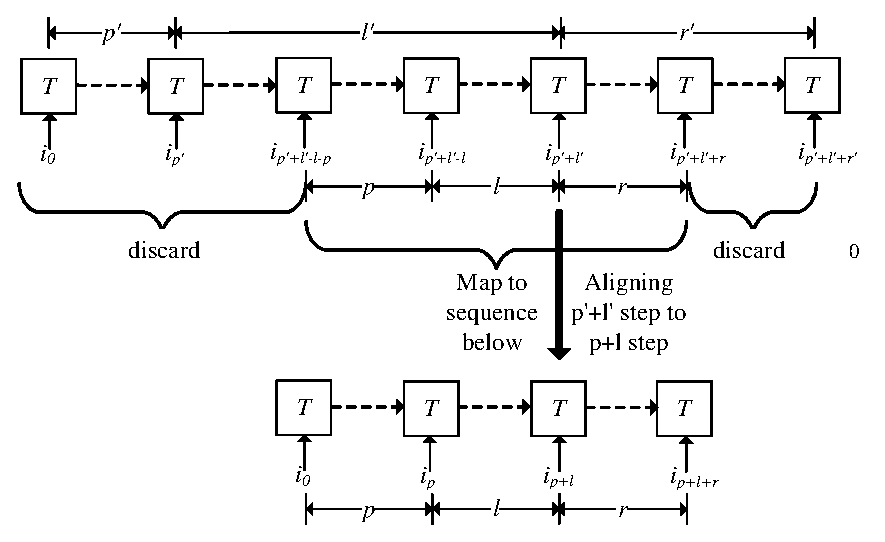
\includegraphics[width=0.7\textwidth]{pcmap}
\end{center}
\caption{通过将第$(p'+l')$步对准第$(p+l)$步映射$F'^d_{PC}(p',l',r',1)$ 到$F'^d_{PC}(p,l,r,1)$。}
  \label{fig_pcmap}
\end{figure}

\begin{figure}[b]
\begin{center}
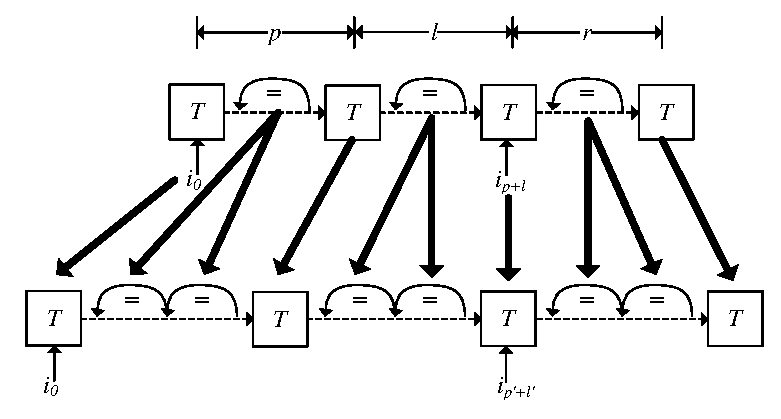
\includegraphics[width=0.7\textwidth]{lnmap}
\end{center}
\caption{通过将第$(p+l)$步对准$(p'+l')$步并展开三个环,从而映射$F'^d_{LN}(p,l,r,1)$ 到$F'^d_{LN}(p',l',r',1)$ 。}
  \label{fig_lnmap}
\end{figure}

\begin{lemma}\label{lemmalninc}
算法\ref{algo_infer} 中的$\mathbf{FSAT_{LN}(p,l,r)}$针对$p$, $l$ 和$r$单调递增。
\end{lemma}
\begin{proof}
对于任意$p'>p$,$l'>l$ 和$r'>l$,
假设$A:\vec{f}_{p+l}\to B$ 是流控变量子在第$(p+l)$步的赋值。
进一步假设$A$ 被$FSAT_{LN}(p,l,r)$覆盖。

因此$A$能够使$F'^d_{LN}(p,l,r,1)$ 可满足。
假设$F'^d_{LN}(p,l,r,1)$ 的可满足赋值为$A'$。
可知$A(\vec{f}_{p+l})\equiv A'(\vec{f}_{p+l})$。

从图\ref{fig_lnmap}可知,
通过对齐第$(p+l)$步到第 $(p'+l')$步,并展开三个环,
我们能将$F'^d_{LN}(p,l,r,1)$ 映射$F'^d_{LN}(p',l',r',1)$ 。
如此可得到$F'^d_{LN}(p',l',r',1)$的可满足赋值$A''$。

通过将$A''$ 的定义域限制为$\vec{f}_{p'+l'}$,
我们可以得到第四个可满足赋值$A''':\vec{f}_{p'+l'}\to B$。
很明显$A\equiv A'''$。

这意味着每个被$FSAT_{LN}(p,l,r)$ 覆盖的赋值也同时被$FSAT_{LN}(p',l',r')$覆盖。
因此$FSAT_{LN}(p,l,r)$ 针对$p$, $l$ 和$r$单调递增。
\end{proof}


\begin{lemma}\label{lemmaln2pc}
$FSAT_{LN}(p,l,r)\Rightarrow FSAT_{PC}(p,l,r)$
\end{lemma}
\begin{proof}
很明显$F'^d_{LN}(p,l,r,1)$ 的短句集合是$F'^d_{PC}(p,l,r,1)$的超集。
所以$F'^d_{LN}(p,l,r,1)$ 的每个可满足赋值也能够使得$F'^d_{PC}(p,l,r,1)$可满足。
因此$FSAT_{LN}(p,l,r)\Rightarrow FSAT_{PC}(p,l,r)$ 成立。
\end{proof}

这三个引理直观的展示在图\ref{fig_mono_chap3}中。
很明显$\neg FSAT_{LN}(p,l,r)\wedge FSAT_{PC}(p,l,r)$ 在算法\ref{algo_infer}中是单调递减的。
基于这些引理,
我们首先证明\ref{algo_infer} 是停机的:

\begin{theorem}
算法\ref{algo_infer} 是停机算法。
\end{theorem}


\begin{proof}
编码器是一个有限状态机,
其最长的无环路径的长度是有限的。
如果算法\ref{algo_infer} 不停机,
则$p$, $l$ 和$r$ 总会大于该长度。
这意味着在下面的三个状态序列$<\vec{s}_{0},\dots,\vec{s}_{p}>$,$<\vec{s}_{p+1},\dots,\vec{s}_{p+l}>$ 和
$<\vec{s}_{p+l+1},\dots,\vec{s}_{p+l+r}>$上必然存在环。
因此,
每个$F'^d_{PC}(p,l,r,1)$ 的可满足赋值必然也能够满足$F'^d_{LN}(p,l,r,1)$。
这意味着$\neg FSAT_{LN}(p,l,r)\wedge FSAT_{PC}(p,l,r)$ 是不可满足的。
这将导致算法\ref{algo_infer}的停机。
所以得证。
\end{proof}


其次,我们将证明算法\ref{algo_infer}的正确性。

\begin{theorem}
从算法\ref{algo_infer}返回的$\neg FSAT_{LN}(p,l,r)$  覆盖且仅覆盖了所有能够使$\vec{d}$
被$\vec{o}$的有限长度序列唯一决定的$\vec{f}$。
\end{theorem}
\begin{proof}
首先证明覆盖的情况。
$FSAT_{LN}(p,l,r)$ 覆盖了一个$\vec{f}$ 集合使得
$\vec{d}$ 对特定的$p$, $l$ 和$r$不能被唯一决定。
因此$\neg FSAT_{LN}(p,l,r)$ 排除了该集合,从而包含了所有能够使得$\vec{d}$被唯一决定的$\vec{f}$。

然后我们证明仅覆盖的情形。
如果$A$是被$\neg FSAT_{LN}(p,l,r)$覆盖的$\vec{f}$的赋值,
且能够使得$\vec{d}$针对特定$p'$, $l'$ 和$r'$不被唯一决定,
则有:

\begin{enumerate}
 \item 一方面$FSAT_{LN}(p',l',r')$也覆盖$A$。
 则从引理\ref{lemmalninc}可知,
 对所有$p''>max(p',p)$,$l''>max(l',l)$ 和$r''>max(r',r)$,
 $FSAT_{LN}(p'',l'',r'')$ 也覆盖$A$。

 \item 同时$FSAT_{LN}(p,l,r)$ 不覆盖 $A$。
 $FSAT_{LN}(p,l,r)$ 是算法\ref{algo_infer} 结束前计算出来的最后一个。
 这意味着$valid(\vec{f})$的上估计和下估计收敛了。
 因此对于所有$p''>max(p',p)$,$l''>max(l',l)$ 和$r''>max(r',r)$,
 $FSAT_{LN}(p'',l'',r'')$ 必然等于$FSAT_{LN}(p,l,r)$。
 因此$FSAT_{LN}(p'',l'',r'')$ 也不覆盖$A$。
\end{enumerate}

这导致了冲突,
因此仅覆盖的情形得证。
\end{proof}


\section{压缩迁移关系展开序列的长度}\label{sec_min}
我们首先在小节\ref{reduceing_chap3}中介绍为什么和如何削减$l$ 和$r$的长度。
然后在小节\ref{alter}中给出我们算法的另一种可能结构。
并讨论为什么我们选择了小节\ref{reduceing_chap3} 中的算法而不是小节\ref{alter}中的算法。

\subsection{压缩$l$ 和$r$}\label{reduceing_chap3}
由于我们在算法\ref{algo_infer}中同步增长$p$,$l$ 和$r$的值。
这导致他们的值有可能包含冗余。
这将导致产生的解码器的面积和时序上有不必要的额外开销。

例如,
假设一个编码器仅包含一个简单的buffer,
其功能为$o:=i$。
当$p\equiv 0$,$l\equiv 0$ 和$r\equiv 0$时,
我们能够得到最简单的解码器$i:=o$。
该解码器只包含一个buffer,而不包含寄存器。而对于$p\equiv 0$,$l\equiv 0$ 和$r\equiv 1$,
我们则需要一个额外的寄存器以将$o$ 延迟一步,
然后从延迟的$o$中回复$i_i$。

根据图\ref{fig_pc_double},
很明显
$r$ 影响解码器的电路面积和延迟,
$l$仅影响解码器的电路面积,
而$p$ 并不对解码器的上述特性带来影响。

因此如算法\ref{algo_remove2_chap3}所示,
我们选择首先压缩$r$,
然后压缩$l$。

\begin{algorithm}[t]
\caption{$RemoveRedundancy(p,l,r)$}
\label{algo_remove2_chap3}
\begin{algorithmic}[1]
\FOR{$r':=r \to 1$}
  \IF{$F_{PC}(p,l,r'-1)\wedge valid(\vec{f}_{p+l})$ 是可满足的}
\label{testr_1}
    \STATE break;
  \ELSIF{$r'\equiv 1$}
\label{testr0}
    \STATE $r':=r'-1$ ;
    \STATE break ;
  \ENDIF
\ENDFOR
\FOR{$l':=l \to 1$}
  \IF{$F_{PC}(p,l'-1,r')\wedge valid(\vec{f}_{p+l'-1})$ 是可满足的}
    \STATE break;
  \ELSIF{$l'\equiv 1$}
    \STATE $l':=l'-1$ ;
    \STATE break;
  \ENDIF
\ENDFOR
\RETURN $<l',r'>$
\end{algorithmic}
\end{algorithm}

为了简化描述,
我们将仅介绍$r$的情况。
在行\ref{testr_1},
当$F_{PC}(p,l,r'-1)\wedge valid(\vec{f}_{p+l})$ 可满足,
则$r'$ 是最后一个使其不可满足的,
我们将其直接返回$r'$。
另一方面,
如果$r'\equiv 0$ 仍能够使行\ref{testr0}的$F_{PC}(p,l,r')\wedge valid(\vec{f}_{p+l})$ 不可满足,
我们直接返回0。

\subsection{另一种可能的算法结构}\label{alter}

在上述讨论中,
我们在算法\ref{alg_fofc_inc}中同步增加$p$, $l$ 和$r$以找到流控变量,
然后在算法\ref{algo_remove2_chap3}中压缩他们的值。
该算法需要调用SAT求解器的次数是$O(n)$ 。
其中$n=max(p,l,r)$。

还有另一种可能的方法:
即使用三个嵌套的环逐一增加$p$, $l$ 和$r$。
该算法需要调用SAT求解器的次数是$O(n^3)$ 。


我们将在小节\ref{subsec_incr_plr_exp} 中指出,
同步增加$p$, $l$ 和$r$ 然后使用算法\ref{algo_remove2_chap3} 进行压缩比单独增加$p$, $l$ 和$r$要更有优势。
我们将在那里对该现象进行解释。





\section{产生解码器函数}\label{sec_char_chap3}
在小节\ref{sec_findfc}中,
解码器的输入$\vec{i}$ 被划分为两个向量:
流控向量$\vec{f}$ 和数据向量$\vec{d}$。
为这两个向量分别产生解码器函数的算法是不同的,
因此他们将在下面两个小节中分别描述。

\subsection{产生$\vec{f}$的解码器函数}\label{subsec_fdec}

每个$f\in \vec{f}$ 都能够被输出向量$\vec{o}$的有限长度序列唯一决定。
所以,
对于每个特定的输出向量序列$<\vec{o}_p,\dots,\vec{o}_{p+l+r}>$,
$f_{p+l}$ 不能同时取值为1和0。
因此,
计算$f_{p+l}$ 的解码器函数可以视为$\phi_A$针对$\phi_B$的Craig插值,
其中$\phi_A$和$\phi_B$分别定义如下:

\begin{equation}\label{fa}
\phi_A:=
\left\{
\begin{array}{cc}
&\bigwedge_{m=0}^{p+l+r}
\{
(\vec{s}_{m+1},\vec{o}_m)\equiv T(\vec{s}_m,\vec{i}_m)
\}
\\
\wedge& f_{p+l}\equiv 1 \\
\wedge&\bigwedge_{m=0}^{p+l+r}assertion(\vec{i}_m)
\end{array}
\right\}
\end{equation}

\begin{equation}\label{fb}
\phi_B:=
\left\{
\begin{array}{cc}
&\bigwedge_{m=0}^{p+l+r}
\{
(\vec{s'}_{m+1},\vec{o'}_m)\equiv T(\vec{s'}_m,\vec{i'}_m)
\}
\\
\wedge&\bigwedge_{m=p}^{p+l+r}\vec{o}_m\equiv \vec{o'}_m \\
\wedge& f'_{p+l}\equiv 0 \\
\wedge&\bigwedge_{m=0}^{p+l+r}assertion(\vec{i'}_m)
\end{array}
\right\}
\end{equation}

显然$\phi_A\wedge \phi_B$ 等价于等式(\ref{uniqt1})中的$F_{PC}(p,l,r)$ ,
因此它是不可满足的。
$\phi_A$ 和$\phi_B$ 的共同变量集合为$<\vec{o}_p,\dots,\vec{o}_{p+l+r}>$。
因此,
Craig插值$ITP$ 可以使用McMillian算法\upcite{interp_McMillan} 从$\phi_A\wedge \phi_B$ 的不可满足证明序列中产生出来。
$ITP$覆盖了所有使得$f_{p+l}\equiv 1$的$<\vec{o}_p,\dots,\vec{o}_{p+l+r}>$的赋值。
同时,
$ITP\wedge \phi_B$ 是不可满足的,
因此$ITP$ 没有覆盖任何使$f_{p+l}\equiv 0$成立的$<\vec{o}_p,\dots,\vec{o}_{p+l+r}>$的赋值。
因此,
$ITP$ 是计算$f\in\vec{f}$的解码函数。

为了进一步提高产生$f\in\vec{f}$的解码函数的速度,
我们通过以下方式使用MiniSat 的递增求解机制:
\begin{enumerate}
 \item
 从$\phi_A$ 中移除$f_{p+l}\equiv 1$,
 从$\phi_B$中移除$f'_{p+l}\equiv 0$。
 \item
 将$\phi_A\wedge \phi_B$ 加入MiniSat的短句数据库。
 \item
 针对每一个$f\in\vec{f}$,
 使用$f_{p+l}\equiv 1$ 和$f'_{p+l}\equiv 0$ 作为求解的假设。
 并从不可满足证明中产生Craig插值。
\end{enumerate}

\subsection{产生$\vec{d}$的解码函数}

假设$valid(\vec{f})$是被算法\ref{algo_infer}推导出来的谓词。
为每个$d\in\vec{d}$,
我们定义以下两个公式:

\begin{equation}\label{da}
\phi_A':=
\left\{
\begin{array}{cc}
&\bigwedge_{m=0}^{p+l+r}
\{
(\vec{s}_{m+1},\vec{o}_m)\equiv T(\vec{s}_m,\vec{i}_m)
\}
\\
\wedge& d_{p+l}\equiv 1 \\
\wedge& valid(\vec{f}_{p+l}) \\
\wedge&\bigwedge_{m=0}^{p+l+r}assertion(\vec{i}_m)
\end{array}
\right\}
\end{equation}

\begin{equation}\label{db}
\phi_B':=
\left\{
\begin{array}{cc}
&\bigwedge_{m=0}^{p+l+r}
\{
(\vec{s'}_{m+1},\vec{o'}_m)\equiv T(\vec{s'}_m,\vec{i'}_m)
\}
\\
\wedge&\bigwedge_{m=p}^{p+l+r}\vec{o}_m\equiv \vec{o'}_m \\
\wedge& d'_{p+l}\equiv 0\\
\wedge& valid(\vec{f'}_{p+l})\\
\wedge&\bigwedge_{m=0}^{p+l+r}assertion(\vec{i'}_m)
\end{array}
\right\}
\end{equation}

当$valid(\vec{f})$ 成立时,
每个$d\in \vec{d}$均能够被唯一决定。
因此,
如果$valid(\vec{f}_{p+l})$ 成立,
对于每个特定的$<\vec{o}_p,\dots,\vec{o}_{p+l+r}>$,
$d_{p+l}$ 不能同时为1和0,
因此,
$\phi_A'\wedge \phi_B'$ 是不可满足的。
因此,
 可以使用McMillian算法\upcite{interp_McMillan} 从$\phi_A'\wedge \phi_B'$的不可满足证明中产生Craig 插值$ITP$。
$ITP$覆盖且仅覆盖使得$d_{p+l}\equiv 1$的$<\vec{o}_p,\dots,\vec{o}_{p+l+r}>$的赋值。
因此,
$ITP$ 是$d\in\vec{d}$的解码器函数。

进一步的
当$valid(\vec{f}_{p+l})$ 不成立时,
数据变量$d\in\vec{d}_{p+l}$ 不能被唯一决定。
因此,
不存在计算它的解码器函数。
不过这并不影响我们的算法的正确性,
因为在这种情况下解码器只需恢复$\vec{f}$,
并忽略$\vec{d}$ 。

类似的,
我们也使用小节\ref{subsec_fdec} 中的增量求解机制加速该算法。



\section{实验结果}\label{sec_exp_chap3}

我们使用OCaml 语言实现了所有算法。
并使用MiniSat 1.14\upcite{EXTSAT}求解所有的CNF公式。
所有的实验使用一台包含16 个Intel Xeon E5648 2.67GHz处理器,
192GB 存储器, 和CentOS 5.4 Linux操作系统的服务器进行。
%All these experimental results and programs can be downloaded
%from https://github.com/shengyushen/compsyn.

\subsection{测试集}
表\ref{tab:summ} 给出了测试集的信息。
他们在自于两个来源:
\begin{enumerate}
 \item 我们以前的论文\upcite{ShenTCAD12}.
 \item Liu et al. \upcite{LiuTCAD12}.
%  \item The benchmark package sent to us by Liu, the author of \upcite{LiuTCAD12}.
%  So there may be some overlap between (2) and (3).
\end{enumerate}

表\ref{tab:summ} 的每一列依次给出了每个实验对象的输入位数,输出位数,状态位数,映射到 mcnc.genlib 标准单元库后的门数和面积。
映射使用ABC 综合工具\upcite{ABC},
脚本为"strash; dsd; strash; dc2; dc2; dch; map"。
该脚本来自于\upcite{LiuTCAD12}。
本文剩余部分给出的所有电路面积和延时都使用同样的设置产生。
这使得我们的结果可以被用于和\upcite{LiuTCAD12}作比较。

\begin{table}[b]%
\caption{Benchmarks}
\label{tab:summ}
\begin{tabular}{|c|c|c|c|c|c|c|}
\hline
                 & 名字      &    个数   &      个数   &电路  & 编码器                               &处理\\
                 &           & in/ouy    &  reg/gate   &面积  &   描述                               & 方法\\\hline\hline
                 & PCIE2     & 10 / 11   & 22   / 149  & 326  &PCIE 2.0                              & 小节                 \\
                 &           &           &             &      &\upcite{pcie21}                       & \ref{subsec_pcie2}         \\\cline{2-7}
 来自于          & XGXS      & 10 / 10   & 17   / 249  & 572  &10Gb以太网                            & 小节                 \\
\upcite{ShenTCAD12}&         &           &             &      & clause 48\upcite{IEEE8023_S4}        & \ref{subsec_10g}           \\\cline{2-7}
并有流控的       & T2Eth     & 14 / 14   & 53   / 427  & 947  &UltraSPARC T2                         & 小节                 \\
测试集           &           &           &             &      & 的以太网模块                         &\ref{subsec_t2e}            \\\hline\hline
                 & XFI       & 72 / 66   & 72   / 5086 & 12381&10Gb以太网                            &                            \\
 来自于\upcite{ShenTCAD12}&  &           &             &      & clause 49\upcite{IEEE8023_S4}        &在小节\ref{subsec_nonflow}                   \\\cline{2-6}
但没有流控的     &SCRAM-     &64/64      &58/353       & 1034 & 增加数据                             &中比较我们的算法                         \\
测试集           &     BLER  &           &             &      & 中的01翻转                           & 和Liu\upcite{LiuTCAD12}\\\cline{1-6}
                 & CC\_3     &   1/3     &   6/22      & 54   &长度为3                               &  \\
                 &           &           &             &      & 的卷机码                             &                          \\\cline{2-6}
                 & CC\_4     &   1/3     &   7/26      & 63   &长度为4                               &                   \\
来自于           &           &           &             &      &的卷机码                              &        \\\cline{2-6}
\upcite{LiuTCAD12}的&HM(7,4) &   4/7     &   3/38      &  103 & 输入4输出7                           &                            \\
测试集           &           &           &             &      & 的汉明码                             &                            \\\cline{2-6}
                 &HM(15,11)  &   11/15   &   4/102     & 317  & 输入11输出15                         &                            \\
                 &           &           &             &      & 的汉明码                             &                            \\\hline
\end{tabular}
\end{table}%

表\ref{tab:summ} 的最后一列
也给出了我们将如何描述每一个benchmark的实验结果。
\begin{enumerate}
 \item
对于来自于我们以前论文\upcite{ShenTCAD12}的5个benchmark,
我们发现他们中的大多数都有流控机制。
这并不奇怪,
因为这些benchmark都来自于实际的工业项目。
他们的实验结果将分别在小节
\ref{subsec_pcie2},\ref{subsec_10g} 和\ref{subsec_t2e}中描述。
 \item
对于其他不包含流控机制的benchmark,
如果他们的输入都能够被输出唯一决定,
则我们的算法能够将他们所有的输入都识别成流控变量,
并直接生成他们的解码器函数。
他们的实验结果将在小节\ref{subsec_nonflow}中描述。
%  \item
% The last two benchmarks in Table \ref{tab:summ} only exist in \upcite{LiuTCAD12}.
% We can not find their source code in the benchmark package sent to us by Liu.
% So we will not discuss them here.
\end{enumerate}

我们还进行了下列额外的实验:

在小节\ref{subsec_incr_plr_exp}中,
我们将比较下列两种不同算法的时间开销:
\begin{enumerate}
 \item 在算法\ref{algo_infer}中同时增长$p$, $l$ 和$r$,
然后在算法\ref{algo_remove2_chap3}中压缩他们的值。
 \item 在算法\ref{algo_infer}中使用三个嵌套的循环分别增长$p$, $l$ 和$r$。
\end{enumerate}

在小节\ref{subsec_min}中,
我们将比较在算法\ref{algo_remove2_chap3}中是否压缩$p$,$l$ 和$r$,
导致的在算法运行时间,解码器面积和延时方面的区别。

最后在小节 \ref{subsec_compareman}中,
我们将比较我们算法产生的解码器和手工书写的解码器在电路面积和延迟方面的差别。


\subsection{PCI Express 2.0 编码器}\label{subsec_pcie2}
该编码器遵从PCI Express 2.0 标准\upcite{pcie21}。
在删除了所有的注释和空行之后,
其源代码包含259 行verilog。

\begin{table}[b]%
\caption{PCI Express 2.0 编码器的输入和输出变量描述}
\label{tab:pcieio}
\centering
\begin{tabular}{|c|c|c|c|}
\hline
         & 变量名               & 宽度  &描述\\\hline\hline
         & $TXDATA$             & 8     &有待编码的数据\\\cline{2-4}
输入     & $TXDATAK$            & 1     &1 意味着$TXDATA$ 是一个控制字符 \\
         &                      &       &0 意味着 $TXDATA$ 是普通数据\\\cline{2-4}
         & $CNTL\_TXEnable\_P0$ & 1     &1意味着$TXDATA$ 和$TXDATAK$的有效性\\\hline
输出     & $HSS\_TXD$           & 10    &被编码的数据\\\cline{2-4}
         & $HSS\_TXELECIDLE$    & 1     &电磁空闲状态\\\hline
\end{tabular}
\end{table}%

表\ref{tab:pcieio}给出了所有输入和输出的描述。
根据8b/10b编码机制的描述\upcite{encode8b10b},
当 $TXDATAK\equiv 0$时,
$TXDATA$ 可以为任何值。
而当$TXDATAK\equiv 1$时,
$TXDATA$ 只能是1C, 3C, 5C, 7C, 9C, BC, DC, FC, F7, FB, FD 和FE。
因此,
我们写了一个断言以剔除不在编码表内的情形,
并将其嵌入迁移函数$T$。

算法\ref{alg_fofc} 在0.475 秒内识别出了流控向量$\vec{f}:=CNTL\_TXEnable\_P0$。
而后算法\ref{algo_infer} 在1.22 秒内推导出了$valid(\vec{f}):=CNTL\_TXEnable\_P0$。
最后算法\ref{algo_remove2_chap3} 在0.69 秒内得到压缩后的$p:=4$, $l:=0$ 和$r:=2$。
最后
产生解码器函数使用了0.26 秒。
最终的解码器包含156 个门和0 个寄存器,
面积为366,
延迟为7.6。


本文算法的创新之处在于其处理流控机制的能力。
我们将展示器编码器如何将无效的数据向量映射到输出向量$\vec{o}$。
通过研究编码器的代码,
我们发现,
当且仅当$CNTL\_TXEnable\_P0\equiv 0$ 成立,
也就是
$TXDATA$ 和$TXDATAK$ 无效时,
输出$HSS\_TXELECIDLE$ 为1.
因此,
解码器将使用$HSS\_TXELECIDLE$ 来唯一决定$CNTL\_TXEnable\_P0$。

\begin{table}[t]%
\caption{10G 以太网编码器XGXS的输入和输出}
\label{tab:eth10g}
\centering
\begin{tabular}{|c|c|c|c|}
\hline
         & 变量名               & 宽度  & 描述\\\hline\hline
         & $encode\_data\_in$   & 8     &将被编码的数据 \\\cline{2-4}
输入     & $konstant$           & 1     &1 意味着 $encode\_data\_in$ 是一个控制字符\\
         &                      &       &0 意味着$encode\_data\_in$ 时普通数据\\\cline{2-4}
         & $bad\_code$          & 1     &1意味着$konstant$ 和$encode\_data\_in$是无效的\\\hline
输出     & $encode\_data\_out$  & 10    &编码结果\\\hline
\end{tabular}
% \begin{tabnote}%
% \Note{Source:}{This is a table
% sourcenote. This is a table sourcenote. This is a table
% sourcenote.}
% \vskip2pt
% \Note{Note:}{This is a table footnote.}
% \tabnoteentry{$^a$}{This is a table footnote. This is a
% table footnote. This is a table footnote.}
% \end{tabnote}%
\end{table}%

\subsection{10G 以太网编码器XGXS}\label{subsec_10g}
该编码器XGXS 遵从IEEE 802.3 标准的\upcite{IEEE8023_S4}的clause 48 。
在删除空行和注释后,
其包含214 行verilog。

表\ref{tab:eth10g}给出了输入和输出变量列表。
该编码器也使用8b/10b 编码机制\upcite{encode8b10b} ,
它包含两个输入:
8位的有待编码数据$encode\_data\_in$ ,
和1位的控制字符标志位$konstant$ 。
根据编码表\upcite{encode8b10b},
当$konstant\equiv 0$时,
$encode\_data\_in$ 可以是任何值。
而当$konstant\equiv 1$时,
$encode\_data\_in$ 只能是1C, 3C, 5C, 7C, 9C, BC, DC, FC, F7, FB, FD 和FE。
因此,
我们将一个手工给出的断言嵌入$T$以剔除不在编码表内的情形。

算法\ref{alg_fofc} 在0.31 秒内识别了流控向量$\vec{f}:=bad\_code$。
然后算法\ref{algo_infer}
在0.95 秒内推导了谓词$valid(\vec{f}):=\!bad\_code$。
再次算法\ref{algo_remove2_chap3} 在0.52 秒内得到压缩结果$p:=4$, $l:=0$ 和$r:=1$。
最后产生解码器使用了0.17 秒。
该解码器包含163 个门和0 个寄存器。
面积为370 ,
延迟为8.1。

虽然该算法使用了和上述PCI Express 2.0 编码器相同的编码机制。
然而它使用了完全不同的方法处理流控机制。
该编码器并没有单独的输出用于表明输出的有效性。
相反,
所有输入的具体值及其有效性都统一编码在$encode\_data\_out$中。
通过研究该编码器的源代码,
我们发现当且仅当$bad\_code\equiv 1$,
既
$encode\_data\_in$ 和$konstant$ 均无效时,
输出变量$encode\_data\_out$ 将成为$0010111101$。
因此解码器能够使用$encode\_data\_out$ 来唯一决定$bad\_code$。



\subsection{UltraSPARC T2 以太网编码器}\label{subsec_t2e}
这个编码器来自于UltraSPARC T2 开源处理器。他遵从于IEEE 802.3 标准\upcite{IEEE8023_S4} 的clause 36。
在删除空行和注释之后,
它包含864 行verilog源代码。


\begin{table}[b]%
\caption{UltraSPARC T2 以太网编码器的输入输出列表}
\label{tab:t2eth}
\centering
\begin{tabular}{|c|c|c|c|}
\hline
         & 变量名字             & 宽度  & 描述\\\hline\hline
         & $txd$                & 8     &有待编码的数据\\\cline{2-4}
输入     & $tx\_enc\_ctrl\_sel$ & 1     &参见表\ref{tab:one} \\\cline{2-4}
         & $tx\_en$             & 1     &传输使能\\\cline{2-4}
         & $tx\_er$             & 1     &传输一个错误字符\\\hline
         & $tx\_10bdata$        & 10    &编码结果 \\\cline{2-4}
         & $txd\_eq\_crs\_ext$  & 10    &传输一个特殊错误字符\\
输出     &                      &       &其中$tx\_er\equiv 1$ 且$txd\equiv 8'h0F$ \\\cline{2-4}
         & $tx\_er\_d$          & 1     &传输一个错误字符\\\cline{2-4}
         & $tx\_en\_d$          & 1     &传输使能\\\cline{2-4}
         & $pos\_disp\_tx\_p$   & 1     &正向parity\\\hline
\end{tabular}
% \begin{tabnote}%
% \Note{Source:}{This is a table
% sourcenote. This is a table sourcenote. This is a table
% sourcenote.}
% \vskip2pt
% \Note{Note:}{This is a table footnote.}
% \tabnoteentry{$^a$}{This is a table footnote. This is a
% table footnote. This is a table footnote.}
% \end{tabnote}%
\end{table}%

表\ref{tab:t2eth}给出了输入和输出变量的列表。
该编码器同样使用8b/10b 编码机制\upcite{encode8b10b},
但是采用了另外一种流控机制,完全不同于上述两个编码器。
有待编码的数据仍然是8位的$txd$。
然而并不存在单独的有效位,
而是在一个4位的$tx\_enc\_ctrl\_sel$ 中定义执行什么样的动作。
细节如表\ref{tab:one}所示。
很明显控制字符和流控机制被混合在$tx\_enc\_ctrl\_sel$中。
表\ref{tab:one} 的最后四种情形不能被唯一决定,
因为他们无法和`PCS\_ENC\_DATA区分开来。
因此我们使用一个断言将他们剔除。

\begin{table}[t]%
\caption{UltraSPARC T2 以太网编码器的动作列表}
\label{tab:one}
\centering
\begin{tabular}{|l|l|}
\hline
动作名称          & 动作含义\\\hline\hline
`PCS\_ENC\_K285   & 发送K28.5 控制字符\\\hline
`PCS\_ENC\_SOP  & 发送 K27.7 控制字符\\\hline
`PCS\_ENC\_T\_CHAR    & 发送 K29.7 控制字符\\\hline
`PCS\_ENC\_R\_CHAR   & 发送 K23.7 控制字符\\\hline
`PCS\_ENC\_H\_CHAR     & 发送 K30.7 控制字符\\\hline
`PCS\_ENC\_DATA     & 发送 编码后的txd\\\hline
`PCS\_ENC\_IDLE2     & 发送 K28.5 D16.2 序列\\\hline
`PCS\_ENC\_IDLE1       & 发送 D5.6 数据符号\\\hline
`PCS\_ENC\_LINK\_CONFA & 发送  K28.5 D21.5 序列\\\hline
`PCS\_ENC\_LINK\_CONFB     & 发送 K28.5 D2.2 序列\\\hline
\end{tabular}
% \begin{tabnote}%
% \Note{Source:}{This is a table
% sourcenote. This is a table sourcenote. This is a table
% sourcenote.}
% \vskip2pt
% \Note{Note:}{This is a table footnote.}
% \tabnoteentry{$^a$}{This is a table footnote. This is a
% table footnote. This is a table footnote.}
% \end{tabnote}%
\end{table}%

算法\ref{alg_fofc} 在3.76 秒内识别了流控信号$\vec{f}:=\{tx\_enc\_ctrl\_sel,tx\_en, tx\_er\}$。
然后算法\ref{algo_infer} 在 21.53 秒内推导了谓词$valid(\vec{f}):=tx\_enc\_ctrl\_sel\equiv `PCS\_ENC\_DATA$。
再次算法\ref{algo_remove2_chap3} 在6.15 秒内得到压缩结果$p:=5$,$l:=0$ 和$r:=4$。
最后产生解码器花费了3.40 秒。
解码器包含401 个门和9 个寄存器。
面积为920 ,
延迟10.2。

如表\ref{tab:one}的最后一列所示,
前5种情况都有各自特殊的控制字符 被赋予$tx\_10bdata$。
因此解码器总能从$tx\_10bdata$恢复出$tx\_enc\_ctrl\_sel$。

\subsection{针对不具备流控机制的编码器比较我们的算法和现有算法}\label{subsec_nonflow}

\begin{table}[b]%
\caption{比较我们的算法和\upcite{LiuTCAD12}的算法}
\centering
\label{tab:comp_nocf}
\begin{tabular}{|c|c|c|c|c|c|c|c|}
\hline
            &\multicolumn{4}{|c|}{我们的算法}                       &\multicolumn{3}{|c|}{\upcite{LiuTCAD12}}\\\cline{2-8}
            &检查解码   & 产生解码& 解码器  & 解码器                &检查解码器          & 解码器  & 解码器\\
名字        & 器存在的  & 器的    & 面积    & 延迟                  & 存在和产生解码     & 面积    & 延迟                \\
            & 时间开销  & 时间开销&         &                       & 器的时间开销       &         &                       \\\hline
XFI         & 13.24     &6.13     & 3878    & 13.8                  & 8.59               &   3913  & 12.5\\\hline
SCRAMBLER   & 1.80      &0.55     & 698     & 3.8                   & 0.42               &   640   & 3.8 \\\hline
 CC\_3      & 0.06      &0.03     & 116     & 8.5                   & 0.21               &   104   & 9.1 \\\hline
 CC\_4      & 0.16      &0.09     & 365     & 12.5                  & 0.20               &   129   & 9.0 \\\hline
 HM(7,4)    & 0.09      &0.03     & 258     & 8.1                   &   0.05             &   255   & 7.3 \\\hline
 HM(15,11)  & 1.49      &2.23     & 5277    & 13.7                  &   2.02             &   3279  & 13.2\\\hline
\end{tabular}
\end{table}%

表\ref{tab:comp_nocf} 针对不具备流控机制的编码器比较了我们的算法和\upcite{LiuTCAD12} 的算法。

%前三个benchmark具备流控机制而且已经在小节\ref{subsec_pcie2},\ref{subsec_10g} 和\ref{subsec_t2e}被讨论过。
%因此他们在这里就不在讨论了。

对于从XFI 到HM(15,11)的6个benchmark,
我们有他们的源代码,
而\upcite{LiuTCAD12} 给出了他们的实验结果。
因此我们能在这里比较我们的算法和\upcite{LiuTCAD12}的结果。

通过比较第二和第三列之和和第六列,
可见\upcite{LiuTCAD12} 比本文算法快很多。
尤其是第二列。
这种差距的主要原因在于本文算法需要逐一检查每个$i\in \vec{i}$ 是否能够被唯一决定,
而\upcite{LiuTCAD12} 可以在一次SAT求解之中检查所有的$\vec{i}$。

另一个问题是本文算法的面积和延迟均大于\upcite{LiuTCAD12},
原因在于本文算法所采用的Craig插值算法实现仍不够优化,
可以通过移植ABC \upcite{ABC}的相应代码得到改善。




\subsection{比较两种可能性:同时增长$p$, $l$ 和$r$ 或者单独增长}\label{subsec_incr_plr_exp}

在算法\ref{alg_fofc_inc}中,
我们同时增加$p$, $l$ 和$r$ ,
并在算法\ref{algo_remove2_chap3}中压缩他们的冗余值。
我们称其为A1方案。

小节\ref{alter} 给出了另一种可能性。
它使用3个嵌套的循环来单独增长每一个$p$, $l$ 和$r$ 。
我们称其为À2方案。

我们在表\ref{tab:comparing_simu_sepa}中比较了这两种方案。

\begin{table}[t]%
\caption{比较两种可能性:同时增长$p$, $l$ 和$r$ 或者单独增长}
\centering
\label{tab:comparing_simu_sepa}
\begin{tabular}{|c|c|c|c|c|c|c|c|c|c|c|}
\hline
                   & \multicolumn{5}{|c|}{A1:同时增长}                          &  \multicolumn{5}{|c|}{A2: 单独增长}           \\\cline{2-11}
benchmarks         & p,l,r& 时间       & 时间            & 时间       &  整体   & p,l,r& 时间       & 时间            & 时间       & 整体  \\
                   &      & 识别       & 推导            & 压缩       &  时间   &      & 识别       & 推导            & 压缩       & 时间   \\
                   &      & $\vec{f}$  & $valid(\vec{f})$& $p$,$l$,$r$&  开下   &      & $\vec{f}$  & $valid(\vec{f})$& $p$,$l$,$r$& 开销   \\\hline\hline
PCIE2              & 3,0,2& 0.49       & 1.21            & 0.68       &  2.38   & 3,0,2& 0.38       & 0.80            & 0.38       & 1.60   \\\hline
XGXS               & 3,0,1& 0.31       & 0.88            & 0.52       &  1.71   & 3,0,1& 0.23       & 0.58            & 0.30       & 1.11   \\\hline
T2Eth              & 4,0,4& 4.28       & 15.17           & 6.25       &  25.70  & 4,0,4& 15.47      & 13.85           & 6.19       & 35.51  \\\hline
XFI                & 2,1,0& 4.59       & 3.60            & 9.55       & 17.74   & 2,1,0& 3.52       & 2.75            & 10.05      & 16.32  \\\hline
SCRAMBLER          & 2,1,0& 0.64       & 0.58            & 1.33       & 2.55    & 2,1,0& 0.48       & 0.43            & 1.47       & 2.38   \\\hline
CC\_3              & 3,2,2& 0.01       & 0.01            & 0.04       & 0.06    & 3,2,2& 0.01       & 0.01            & 0.01       & 0.03   \\\hline
CC\_4              & 4,4,3& 0.07       & 0.01            & 0.08       & 0.16    & 4,1,4& 0.16       & 0.01            & 0.07       & 0.25   \\\hline
HM(7,4)            & 3,0,0& 0.02       & 0.01            & 0.07       & 0.09    & 3,0,0& 0.01       & 0.01            & 0.04       & 0.06   \\\hline
HM(15,11)          & 3,0,0& 0.22       & 0.05            & 1.21       & 1.49    & 3,0,0& 0.34       & 0.04            & 0.58       & 0.96   \\\hline
\end{tabular}
\end{table}%

通过比较第6 和11列中的整体时间开销,
很显然
A2 在大多数情形下比A1 快。
只有T2Eth是一个例外。

这意味着我们应当使用A2 而不是A1吗?
答案是否定的。

从小节\ref{alter}可知,
A1需要调用SAT求解器的次数为$O(n)$ ,
其中$n=max(p,l,r)$。
而A2需要的次数为$O(n^3)$ 。
对于比较小的$n$,
两者并没有很大的区别。
而对于较大的$n$,
比如T2Eth,
A1对A2的优势是显著的。

因此A2在小电路上有优势,
而A1 在大电路上有优势。
因此我们仍然选择A1。
也就是首先同步增加$p$, $l$ 和$r$ ,
然后在算法\ref{algo_remove2_chap3}中压缩他们。

CC\_4 是唯一一个在第2列和第7列具有不同$p$,$l$和$r$的benchmark。
这是由于$l$ 和$r$的不同增长顺序导致的。
对于A1 方案,
其解码器包含14 个寄存器, 206 个门, 490 面积和13.3 延迟。
对于A2 方案,
其解码器包含10 个寄存器, 61 个门, 154 面积和9.6 延迟。
因此A2 方案比A1好很多。
但是这仍然不意味着我们应当使用A2。
具体原因我们将在下一小节得到更多实验数据支撑之后进一步展开解释。

\subsection{在压缩和不压缩$l$ 和$r$的两种算法之间比较运行时间,电路面积和延迟}\label{subsec_min}

\begin{table}[t]%
\caption{在压缩和不压缩$l$ 和$r$的两种算法之间比较运行时间,电路面积和延迟}
\label{tab:compare_min}
\centering
\begin{tabular}{|c|c|c|c|c|c|c|c|c|c|c|c|c|}
\hline
            & \multicolumn{5}{|c|}{不压缩} &  \multicolumn{6}{|c|}{使用算法\ref{algo_remove2_chap3}压缩} \\\cline{2-12}
bench-      & p,l,r& 时间       & 解码    & 寄存& 最大                                      &时间        & p,l,r& 时间       &解码     & 寄存&最大\\
marks       &      & 生成       & 器      & 器  &  逻辑                                     &压缩        &      & 生成       & 器      & 器  &逻辑            \\
            &      & 解码器     &  面积   & 个数&延迟                                       &$p$,$l$,$r$ &      & 解码器     &  面积   & 个数& 延迟\\\hline\hline
PCIE2       & 3,3,3& 0.44       &  382    & 11  & 7.5                                       &0.68        & 3,0,2& 0.28       &  366    & 0   & 7.6             \\\hline
XGXS        & 3,3,3& 0.35       &  351    &20   &8.2                                        &0.52        & 3,0,1& 0.18       &  370    & 0   & 8.1             \\\hline
T2Eth       & 4,4,4& 4.76       &  1178   & 9   & 10.9                                      &6.25        & 4,0,4& 3.41       &  920    & 9   & 10.2            \\\hline
XFI         & 2,2,2& 10.67      & 5079    &190  & 16.50                                     &9.55        & 2,1,0& 6.13       &  3878   & 58  & 13.8            \\\hline
SCRMBL      & 2,2,2& 1.27       & 826     &186  &  3.8                                      &1.33        & 2,1,0& 0.55       &  698    & 58  & 3.8             \\\hline
CC\_3       & 3,3,3& 0.04       &  117    & 11  & 9.2                                       &0.04        & 3,2,2& 0.03       &  116    & 9   & 8.5             \\\hline
CC\_4       & 4,4,4& 0.05       & 154     & 10  & 9.6                                       &0.08        & 4,4,3& 0.09       &  365    & 14  & 12.5            \\\hline
HM(7,4)     & 3,3,3& 0.05       & 262     & 21  & 7.2                                       &0.07        & 3,0,0& 0.03       &  258    & 0   & 8.1             \\\hline
HM(15,11)   & 3,3,3& 2.98       & 5611    & 45  & 13.5                                      &1.21        & 3,0,0& 2.23       &  5277   & 0   & 13.7            \\\hline
\end{tabular}
\end{table}%

为了改善解码器的面积和延迟,
算法\ref{algo_remove2_chap3} 被用于在产生解码器之前压缩$l$ 和$r$。
表\ref{tab:compare_min}展示了其效果。

第一列是benchmark名字。
当算法\ref{algo_remove2_chap3} 没有被使用时,
第2列到第6列分别给出了$p$,$l$ 和$r$ 的值,
产生解码器的运行时间,
解码器面积,
解码器包含的寄存器个数,
解码器最大的逻辑延迟。
当算法\ref{algo_remove2_chap3} 被使用的时候,
这些数据在最后5列给出。
而第7列给出了$l$ 和$r$。

通过比较2-6 列和8-12 列,
很明显算法\ref{algo_remove2_chap3}显著的压缩了$l$ 和$r$ 。

CC\_4 再次引起我们的注意。
从第4列到第6列,
我们发现电路面积和延迟非常类似于上一小节的A2情形。
而他的$p$,$l$ 和$r$ 则类似于A1 情形。
这意味着分CC\_4 的解码器有至少两种差别很大的实现方式。
而具体哪一种被选中取决于SAT求解器和Craig插值算法内部的某些不稳定因素。
这回答了我们在上一小节的疑惑,
即A1方案中的电路质量下降并不是由A1导致的。
我们仍然应当使用À1。


\subsection{在我们的算法和手工书写的解码器之间比较电路面积和延迟}\label{subsec_compareman}

\begin{table}[b]%
\caption{在我们的算法和手工书写的解码器之间比较电路面积和延迟}
\label{tab:comparing_hand}
\centering
\begin{tabular}{|c|c|c|c|c|c|c|c|c|c|c|c|}
\hline
bench-   & \multicolumn{2}{|c|}{本文算法} &  \multicolumn{2}{|c|}{手工书写的解码器} \\\cline{2-5}
marks    & 面积    & 最大逻辑演出       &面积    & 最大逻辑延迟\\\hline
PCIE2    & 366     &7.6                 & 594    & 9.7                              \\\hline
XGXS     & 370     &8.1                 & 593    & 11.0                             \\\hline
T2Eth    & 920     &10.2                & 764    & 11.7                             \\\hline
XFI      & 3878    & 13.8               & 3324   & 28.1                             \\\hline
SCRAMBLER& 698     & 3.8                & 1035   & 6.4                              \\\hline
%  CC\_3   & \multicolumn{4}{|c|}{}\\\cline{1-1}
%  CC\_4   & \multicolumn{4}{|c|}{No manually written Decoder to be compared with.}\\\cline{1-1}
% HM(7,4)  & \multicolumn{4}{|c|}{}\\\cline{1-1}
% HM(15,11)& \multicolumn{4}{|c|}{}\\\hline
\end{tabular}
\end{table}%

表\ref{tab:comparing_hand} 在我们的算法和手工书写的解码器之间比较电路面积和延迟。
CC\_3,CC\_4, HM(7,4) and HM(15,11) 没有
在该表中是因为我们没有他们的手写解码器。

很明显在大多数情况下我们的解码器比手工解码器更小也更快。
少数的两个例外是T2Eth 和XFI ,
我们产生的解码器比手工解码器稍微大一些。



\section{结论}\label{sec_conclude_chap3}

本文提出了第一个能够处理流控机制的对偶综合算法。
实验结果表明本文算法能够为多个来自于实际工业项目的复杂编码器,
包括PCI Express \upcite{pcie21} 和以太网\upcite{IEEE8023_S4}。


